\newpage
\chapter{TINJAUAN PUSTAKA} \label{Bab II}

\section{Tinjauan Pustaka} \label{II.Tinjauan}
Penelitian dalam bidang penerjemahan dan pengenalan Sistem Isyarat Bahasa Indonesia (SIBI) telah banyak dilakukan dengan berbagai pendekatan untuk meningkatkan akurasi dan efisiensi sistem. Beragam studi berfokus pada pengolahan fitur visual, baik melalui ekstraksi bentuk tangan, kerangka tubuh, maupun penggabungan keduanya. Seiring perkembangan teknologi \textit{deep learning}, muncul pendekatan berbasis \textit{transfer learning} dan arsitektur \textit{Transformer} yang mampu mempelajari hubungan kompleks antar-komponen visual dan linguistik secara simultan. Beberapa penelitian yang relevan dengan topik ini dijelaskan berikut sebagai dasar konseptual dan pembanding bagi penelitian yang dilakukan. \par


\begin{enumerate}[noitemsep]
	\item Carreira dan Zisserman \cite{Carreira2017I3D} memperkenalkan I3D (\textit{Inflated 3D ConvNets}) sebagai arsitektur pengenalan aksi berbasis video yang mengembangkan filter dua dimensi dari jaringan Inception-V1 pralatih menjadi filter tiga dimensi, sehingga informasi spasial dan temporal dapat dipelajari secara \textit{end-to-end}. Teknik \textit{inflation} ini memungkinkan model memanfaatkan bobot pralatih ImageNet sebagai titik awal yang baik sebelum dilanjutkan dengan pralatih pada Kinetics-400. I3D mencapai akurasi \textit{state-of-the-art} pada UCF-101 dan HMDB-51, menjadikannya \textit{baseline} 3D CNN yang kuat dan banyak dijadikan rujukan dalam evaluasi sistem pengenalan aksi maupun pengenalan bahasa isyarat berbasis video \cite{Carreira2017I3D}.

	\item Arnab dkk.\ \cite{Arnab2021} memperkenalkan \textit{Video Vision Transformer} (ViViT) sebagai arsitektur berbasis Transformer murni untuk pemahaman video. ViViT memperluas \textit{Vision Transformer} (ViT) ke domain video dengan membagi video menjadi token spasio-temporal melalui \textit{tubelet embedding}, kemudian memodelkan ketergantungan antar-token menggunakan \textit{self-attention} tanpa komponen konvolusi. Dilatih secara \textit{supervised} pada Kinetics-400 dan JFT, ViViT mencapai performa kompetitif pada beberapa \textit{benchmark} video dan mewakili paradigma \textit{supervised video transformer} yang berbeda secara fundamental dari I3D maupun pendekatan \textit{self-supervised} \cite{Arnab2021}.

	\item Alsraisri \cite{Alsraisri2025} melalui penelitian berjudul ``\textit{Achieving State-of-the-art Accuracy in Arabic Sign Language Recognition with VideoMAE and Data Augmentation}'' menunjukkan bahwa VideoMAE (\textit{Video Masked Autoencoder}) efektif untuk pengenalan bahasa isyarat berbasis video. Penelitian ini menerapkan VideoMAE yang dipadukan dengan strategi augmentasi data untuk klasifikasi \textit{Arabic Sign Language} (ArSL) dan berhasil mencapai akurasi \textit{state-of-the-art}, membuktikan potensi VideoMAE sebagai model \textit{video Transformer self-supervised} untuk tugas pengenalan bahasa isyarat pada dataset yang relatif terbatas \cite{Alsraisri2025}.

	\item Studi oleh Rakun dan Setyono \cite{RakunSetyono2022} berjudul ``\textit{Improving Recognition of SIBI Gesture by Combining Skeleton and Hand Shape Features}'' mengusulkan metode pengenalan bahasa isyarat SIBI dengan menggabungkan dua representasi visual, yaitu fitur kerangka tubuh (\textit{skeleton}) dan bentuk tangan (\textit{hand shape}). Penelitian ini menggunakan metode \textit{pose estimation} dengan \textit{OpenPose} untuk mengekstraksi koordinat titik sendi tubuh seperti bahu, siku, dan pergelangan tangan, sedangkan bentuk tangan dianalisis melalui CNN guna menangkap pola spasial jari. Kedua fitur tersebut difusikan menggunakan teknik \textit{sequence-feature-vector concatenation} dan diklasifikasikan dengan LSTM serta GRU untuk memodelkan urutan waktu. Hasil pengujian menunjukkan akurasi sebesar 88.02\%, yang membuktikan bahwa kombinasi dua fitur visual mampu meningkatkan akurasi pengenalan isyarat tangan, meskipun belum mempertimbangkan ekspresi wajah atau elemen non-manual lain yang berperan penting dalam komunikasi isyarat. \par
	\item Penelitian selanjutnya oleh Rakun dkk. \cite{RakunDarmana2022} berjudul ``\textit{SIBI (Sign System Indonesian Language) Text-to-3D Animation Translation Model Using Deep Learning and Pose Estimation}'' berfokus pada pengembangan sistem penerjemahan teks ke animasi 3D bahasa isyarat atau \textit{text-to-sign translation}. Sistem ini menggabungkan metode \textit{pose estimation} dengan \textit{3D animation generator} untuk menghasilkan \textit{avatar} virtual yang mampu menirukan gerakan tangan dan ekspresi bibir secara sinkron. Metode CNN digunakan untuk mengonversi teks menjadi parameter gerakan berupa \textit{joint angles} dan \textit{lip shapes}. Hasil penelitian menunjukkan sistem mampu menghasilkan animasi bahasa isyarat yang lebih alami dan sinkron, namun masih terbatas karena belum mendukung penerjemahan dua arah serta belum mengintegrasikan modalitas non-manual seperti ekspresi wajah nyata.
	\item Pratama dkk. \cite{Pratama2025} melalui penelitian berjudul ``Model \textit{Deep Learning} untuk Penerjemah Bahasa Isyarat SIBI dengan Arsitektur \textit{Transfer Learning}'' mengembangkan sistem penerjemah bahasa isyarat berbasis \textit{deep learning} dengan menerapkan \textit{transfer learning} menggunakan arsitektur \textit{MobileNetV2} sebagai ekstraktor fitur visual. Hasil vektor fitur kemudian diolah menggunakan LSTM untuk mengenali urutan gerakan dan menerjemahkannya menjadi teks. Hasil pengujian menunjukkan bahwa model ini mampu mencapai keseimbangan antara akurasi dan efisiensi komputasi, sehingga memungkinkan penerapan pada perangkat bergerak. Namun, karena hanya mengandalkan sinyal visual, sistem ini masih memiliki kelemahan dalam membedakan isyarat dengan bentuk tangan mirip yang memiliki konteks makna berbeda.
	\item Nugraha dan Rakun \cite{MHNugraha2022} dalam penelitian berjudul ``\textit{Solving Complex Background Problem Using RetinaNet for Sign System for Indonesian Language (SIBI) Gesture-to-Text Translator}'' menyoroti permasalahan latar belakang kompleks dalam video bahasa isyarat. Penelitian ini menggunakan metode \textit{RetinaNet} berbasis \textit{Feature Pyramid Network (FPN)} dan \textit{Focal Loss} untuk meningkatkan akurasi deteksi area tangan pada berbagai kondisi skala dan pencahayaan. Hasil penelitian menunjukkan bahwa pendekatan ini berhasil meningkatkan stabilitas proses ekstraksi fitur dan memberikan kontribusi penting pada tahap pra-pemrosesan visual sebelum tahap penerjemahan bahasa isyarat dilakukan.
	\item Aurelrius dkk. \cite{Aurelrius2025} dalam penelitian berjudul ``\textit{Transfer Learning and Custom Loss Applied to Transformer-Based Text Translation for Sign Language Animated Subtitles}'' mengimplementasikan arsitektur \textit{Transformer} untuk penerjemahan teks ke animasi bahasa isyarat. Penelitian ini menerapkan \textit{transfer learning} dan \textit{custom loss function} yang dirancang untuk menjaga keselarasan temporal antar-frame dalam animasi. Metode \textit{self-attention} pada \textit{Transformer} digunakan untuk mempelajari hubungan antar-kata dalam teks dan gerakan tangan dalam animasi. Hasil pengujian menunjukkan peningkatan signifikan dalam sinkronisasi subtitle teks dengan animasi dibandingkan pendekatan berbasis RNN, meskipun model ini belum mencakup pengenalan langsung dari video isyarat.

	\item Camgoz et al. \cite{NCCamgoz2021} melalui penelitian ``\textit{Multi-Channel Transformers for Multi-Articulatory Sign Language Translation}'' memperkenalkan arsitektur \textit{Transformer} dengan saluran ganda (\textit{multi-channel}) untuk penerjemahan bahasa isyarat kontinu menjadi teks. Model ini memisahkan representasi untuk tangan, wajah, dan tubuh, yang kemudian digabungkan menggunakan \textit{multi-head attention}. Hasil penelitian menunjukkan peningkatan akurasi dibandingkan model CNN-LSTM konvensional karena model mampu menangkap hubungan antarkomponen artikulator secara paralel serta memproses dependensi jangka panjang antara gestur dan urutan kata target.
	\item Zhou et al. \cite{Zhou2021} dalam penelitian ``\textit{Improving Sign Language Translation with Monolingual Data by Sign Back-Translation}'' mengusulkan pendekatan augmentasi data monolingual menggunakan teknik \textit{sign back-translation}. Metode ini menghasilkan data tambahan dengan menerjemahkan teks menjadi isyarat kemudian kembali ke teks menggunakan \textit{Transformer}, sehingga menciptakan korpus pelatihan baru tanpa memerlukan pasangan data paralel dalam jumlah besar. Hasil penelitian menunjukkan bahwa teknik ini mampu meningkatkan performa model pada dataset Phoenix-2014T dan memperluas kemampuan generalisasi sistem penerjemahan bahasa isyarat.

\end{enumerate}

Sebagai pelengkap dari uraian sebelumnya, Tabel 2.1 berikut merangkum hasil tinjauan pustaka terhadap beberapa penelitian terdahulu, mencakup penulis, judul, permasalahan dan metode serta hasil. \par
\clearpage
\begin{landscape}
{\small
\setlength{\tabcolsep}{3pt}
\newlength{\literatureTableWidth}
\setlength{\literatureTableWidth}{\dimexpr\linewidth-12\tabcolsep-7\arrayrulewidth\relax}% 6 kolom = 12\tabcolsep, 7 garis vertikal
\begin{longtable}{|>{\raggedleft\arraybackslash}p{0.06\literatureTableWidth}|>{\raggedright\arraybackslash}p{0.17\literatureTableWidth}|>{\raggedright\arraybackslash}p{0.21\literatureTableWidth}|>{\raggedright\arraybackslash}p{0.15\literatureTableWidth}|>{\raggedright\arraybackslash}p{0.23\literatureTableWidth}|>{\raggedright\arraybackslash}p{0.18\literatureTableWidth}|}
\caption{Literasi Penelitian Terdahulu}\label{table:2.literasi}\\
\hline
\rowcolor{gray!15} \multicolumn{1}{|c|}{No.} & \multicolumn{1}{c|}{Penulis} & \multicolumn{1}{c|}{Judul} & \multicolumn{1}{c|}{Masalah} & \multicolumn{1}{c|}{Metode} & \multicolumn{1}{c|}{Hasil} \\
\hline
\endfirsthead

\multicolumn{6}{c}{\tablename\ \thetable\, \textit{Lanjutan dari halaman sebelumnya}} \\
\hline
\rowcolor{gray!15} \multicolumn{1}{|c|}{No.} & \multicolumn{1}{c|}{Penulis} & \multicolumn{1}{c|}{Judul} & \multicolumn{1}{c|}{Masalah} & \multicolumn{1}{c|}{Metode} & \multicolumn{1}{c|}{Hasil} \\
\hline
\endhead

\hline
\multicolumn{6}{r}{\textit{Bersambung ke halaman berikutnya}} \\
\endfoot

\hline
\endlastfoot

1. & J. Carreira \& A. Zisserman \cite{Carreira2017I3D} & \textit{Quo Vadis, Action Recognition? A New Model and the Kinetics Dataset} & Pemodelan video memerlukan representasi spasio-temporal yang kuat tanpa kehilangan manfaat bobot pra-latih citra. & I3D (\textit{Inflated 3D ConvNets}): filter 2D Inception-V1 di-\textit{inflate} ke 3D, pra-latih pada Kinetics-400. & Akurasi \textit{state-of-the-art} pada UCF-101 dan HMDB-51; I3D menjadi \textit{baseline} 3D CNN yang kuat untuk pengenalan aksi dan bahasa isyarat berbasis video. \\
\hline

2. & A. Arnab et al. \cite{Arnab2021} & \textit{ViViT: A Video Vision Transformer} & Pemodelan video memerlukan arsitektur yang mampu menangkap dependensi spasio-temporal secara global tanpa konvolusi. & \textit{Video Vision Transformer} (ViViT): video dibagi menjadi token spasio-temporal via \textit{tubelet embedding}, dimodelkan dengan \textit{self-attention}, dilatih \textit{supervised} pada Kinetics-400 dan JFT. & Performa kompetitif pada beberapa \textit{benchmark} video; ViViT mewakili paradigma \textit{supervised video transformer} yang berbeda dari 3D CNN maupun model \textit{self-supervised}. \\
\hline

3. & N. Alsraisri \cite{Alsraisri2025} & \textit{Achieving State-of-the-art Accuracy in Arabic Sign Language Recognition with VideoMAE and Data Augmentation} & Pengenalan bahasa isyarat berbasis video memerlukan model yang mampu menangkap pola spasio-temporal secara akurat pada data berlabel terbatas. & VideoMAE (\textit{self-supervised video transformer}) dipadukan dengan strategi augmentasi data untuk klasifikasi \textit{Arabic Sign Language} (ArSL). & Mencapai akurasi \textit{state-of-the-art}; VideoMAE terbukti efektif untuk pengenalan bahasa isyarat berbasis video dengan pemodelan spasio-temporal yang kuat pada dataset terbatas. \\
\hline

4. & E. Rakun \& N. Setyono \cite{RakunSetyono2022} & \textit{Improving Recognition of SIBI Gesture by Combining Skeleton and Hand Shape Features} & Keterbatasan penggunaan fitur tunggal dalam mengenali isyarat SIBI yang ambigu. & Penggabungan fitur \textit{skeleton} dan \textit{hand shape} menggunakan \textit{OpenPose} dan CNN, diklasifikasikan dengan RNN LSTM atau GRU. & Akurasi hingga 88.02\% dan fusi fitur efektif. \\
\hline

5. & E. Rakun et al. \cite{RakunDarmana2022} & \textit{SIBI Text-to-3D Animation Translation Model Using Deep Learning and Pose Estimation} & Belum ada sistem interaktif yang menerjemahkan teks ke animasi bahasa isyarat. & Model \textit{deep learning} dengan ekstraksi pose \textit{OpenPose} dan sistem animasi 3D sinkron dengan gerakan bibir. & Sistem teks ke animasi 3D yang akurat dan sinkron. \\
\hline

6. & M. H. Nugraha \& E. Rakun \cite{MHNugraha2022} & \textit{Solving Complex Background Problem Using RetinaNet for SIBI Gesture-to-Text Translator} & Deteksi tangan gagal pada latar kompleks. & \textit{RetinaNet} berbasis \textit{FPN} dan \textit{Focal Loss} untuk deteksi area tangan dan tubuh. & Akurasi deteksi dan stabilitas pengenalan meningkat. \\
\hline

7. & F. Pratama et al. \cite{Pratama2025} & \textit{Model Deep Learning untuk Penerjemah Bahasa Isyarat SIBI dengan Arsitektur Transfer Learning} & Tantangan model efisien namun akurat. & \textit{Transfer learning} CNN \textit{MobileNetV2} untuk fitur visual dan LSTM untuk urutan gerakan. & Efisien untuk mobile dan akurat. \\
\hline

8. & E. Aurelrius et al. \cite{Aurelrius2025} & \textit{Transfer Learning and Custom Loss Applied to Transformer-Based Text Translation for Sign Language Animated Subtitles} & Butuh sinkronisasi alami antara teks dan animasi. & \textit{Transformer} dengan \textit{transfer learning} dan \textit{custom loss} untuk menjaga kesesuaian temporal. & Sinkronisasi waktu dan transisi gerakan membaik. \\
\hline

9. & N. C. Camgoz et al. \cite{NCCamgoz2021} & \textit{Multi-Channel Transformers for Multi-Articulatory Sign Language Translation} & Sulit menangkap hubungan antar komponen tubuh. & \textit{Multi-Channel Transformer} untuk tangan, wajah, tubuh digabung via \textit{multi-head attention}. & Akurasi sign-to-text meningkat. \\
\hline

10. & H. Zhou et al. \cite{Zhou2021} & \textit{Improving Sign Language Translation with Monolingual Data by Sign Back-Translation} & Keterbatasan data paralel video-teks. & \textit{Sign back-translation} dengan \textit{Transformer} untuk data monolingual tambahan. & Performa meningkat pada Phoenix-2014T dan generalisasi lebih baik. \\
\hline

\end{longtable}
}
\end{landscape}
\clearpage

\section{Dasar Teori} \label{II.Teori}


\subsection{Bahasa Isyarat} \label{II.Teori1}
Bahasa isyarat merupakan sistem komunikasi visual-gestural yang digunakan oleh komunitas Tuli untuk menyampaikan makna melalui gerakan tangan, bentuk jari, ekspresi wajah, serta gerakan tubuh \cite{Saputra2024}. Bahasa ini memiliki struktur linguistik sendiri yang mencakup fonologi manual, morfologi, sintaksis, dan semantik, berbeda dengan bahasa lisan yang berbasis suara \cite{RakunWidhinugraha2022}.\par
Secara global, penelitian bahasa isyarat telah berkembang dari sisi linguistik dan teknologi. Kajian terbaru menunjukkan bahwa bahasa isyarat memiliki kompleksitas visual tinggi dan menuntut representasi spasial-temporal yang kaya agar dapat diproses secara akurat \cite{Saputra2024}. Di Indonesia sendiri, terdapat dua sistem utama bahasa isyarat yang digunakan, yaitu Sistem Isyarat Bahasa Indonesia (SIBI) dan Bahasa Isyarat Indonesia (BISINDO) \cite{Ratriyana2022}.\par
	
	% \begin{longtable}{|c|c|c|c|}
	% 	\caption{Contoh Tabel}
	% 	\label{table:2.contoh}\\
	% 	\hline
	% 	Col1 & Col2 & Col2 & Col3 \\
	% 	\hline
	% 	\endhead
	% 	1 & 6 & 87837 & 787 \\ 
	% 	\hline
	% 	2 & 7 & 78 & 5415 \\
	% 	\hline
	% 	3 & 545 & 778 & 7507 \\
	% 	\hline
	% 	4 & 545 & 18744 & 7560 \\
	% 	\hline
	% 	5 & 88 & 788 & 6344 \\
	% 	\hline
	% \end{longtable}

\subsubsection{Sistem Isyarat Bahasa Indonesia (SIBI)} \label{II.Teori1.1}
Sistem Isyarat Bahasa Indonesia (SIBI) merupakan sistem komunikasi visual yang dirancang secara buatan oleh pemerintah Indonesia sebagai sarana pembelajaran dan komunikasi formal bagi penyandang Tuli \cite{RakunSetyono2022}. Sistem ini juga digunakan dalam konteks pendidikan formal karena pengembangannya mengikuti standar komunikasi resmi \cite{RakunDarmana2022}. SIBI dikembangkan untuk menyesuaikan tata bahasa Bahasa Indonesia ke dalam bentuk isyarat manual yang terstruktur dan mudah dipahami oleh peserta didik tunarungu \cite{RakunDarmana2022}. Penerapannya menjadi standar di Sekolah Luar Biasa agar siswa Tuli dapat memahami Bahasa Indonesia secara tertulis melalui gerakan tangan dan simbol visual \cite{Zulpicha2017}.\par

Secara linguistik, SIBI mengikuti struktur gramatikal Bahasa Indonesia, termasuk urutan kata, imbuhan, dan partikel tata bahasa \cite{RakunSetyono2022}. Setiap unsur linguistik direpresentasikan oleh simbol tangan atau gerakan tertentu yang mengikuti pola subjek–predikat–objek \cite{Pratama2025}. Sistem ini dinilai efektif untuk pembelajaran bahasa pada anak tunarungu karena bentuknya yang terstruktur \cite{Zulpicha2017}. Namun struktur SIBI dianggap kurang alami dalam komunikasi sehari-hari karena tidak menekankan unsur nonverbal seperti ekspresi wajah atau gerakan tubuh \cite{RakunDarmana2022}. Unsur-unsur nonverbal ini memiliki peran penting dalam memperjelas makna dan emosi, terutama dalam interaksi natural komunitas Tuli \cite{Ratriyana2022}.\par

Unsur nonverbal atau nonmanual dalam bahasa isyarat berfungsi seperti intonasi dalam bahasa lisan \cite{Saputra2024}. Ekspresi wajah, arah pandangan, dan gerakan alis memberikan konteks emosional dan gramatikal tambahan \cite{RakunWidhinugraha2022}. Pada SIBI, aspek tersebut kurang ditekankan karena fokusnya pada struktur formal Bahasa Indonesia. Penelitian terbaru mulai mengintegrasikan fitur nonverbal ke dalam sistem pengenalan bahasa isyarat berbasis \textit{deep learning} untuk meningkatkan kealamian gerakan dan pemahaman semantik \cite{RakunDarmana2022}. Integrasi ini juga membantu meningkatkan kemampuan sistem dalam mengenali ekspresi dan variasi gerakan yang lebih kompleks \cite{MHNugraha2022}.\par

\begin{figure}[H]
	\centering
	\begin{subfigure}{0.48\textwidth}
		\centering
		\fbox{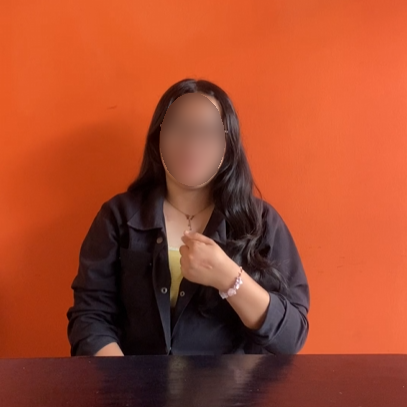
\includegraphics[width=0.75\textwidth]{figure/aku.png}}
		\caption{Isyarat SIBI kata aku}
	\end{subfigure}
	\hfill
	\begin{subfigure}{0.48\textwidth}
		\centering
		\fbox{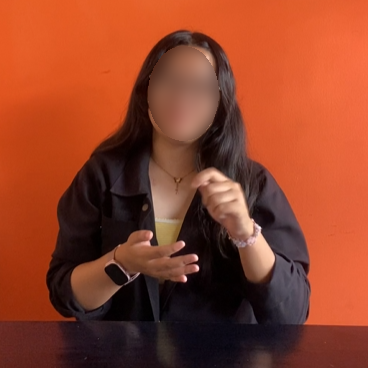
\includegraphics[width=0.75\textwidth]{figure/sekolah.png}}
		\caption{Isyarat SIBI kata sekolah}
	\end{subfigure}
	\caption[Contoh gerakan Sistem Isyarat Bahasa Indonesia (SIBI) dari dataset penelitian]{Contoh gerakan Sistem Isyarat Bahasa Indonesia (SIBI) dari dataset penelitian}
	\label{fig:2.sibi&bisindo}
	{\footnotesize Sumber: Data primer penelitian\par}
\end{figure}

Berbeda dengan SIBI, Bahasa Isyarat Indonesia (BISINDO) merupakan bahasa alami (\textit{natural sign language}) yang berkembang secara organik di komunitas Tuli \cite{Ratriyana2022}. Struktur BISINDO tidak mengikuti tata bahasa Bahasa Indonesia, melainkan mengandalkan konteks visual, ekspresi wajah, dan gerakan tubuh untuk menyampaikan makna secara langsung. Oleh karena itu, BISINDO bersifat lebih ekspresif dan kontekstual, sedangkan SIBI lebih terstruktur dan formal. Perbedaan utama antara keduanya terletak pada orientasi fungsional: SIBI digunakan dalam konteks pendidikan dan komunikasi resmi, sementara BISINDO digunakan dalam interaksi sosial sehari-hari di komunitas Tuli \cite{Zulpicha2017}. Untuk memberikan gambaran yang lebih jelas mengenai perbedaan kedua sistem tersebut, Tabel~\ref{table:2.perbandingan} berikut memperlihatkan perbandingan antara BISINDO dan SIBI berdasarkan beberapa aspek linguistik dan penggunaannya.\par

\begingroup
\setlength{\tabcolsep}{8pt}
\renewcommand{\arraystretch}{1.4}
\begin{longtable}{|>{\raggedright\arraybackslash}p{0.17\textwidth}|>{\raggedright\arraybackslash}p{0.37\textwidth}|>{\raggedright\arraybackslash}p{0.31\textwidth}|}
	\caption{Perbedaan BISINDO dan SIBI}
	\label{table:2.perbandingan}\\
	\hline
	\rowcolor{gray!15} \multicolumn{1}{|c|}{\textbf{Aspek}} & \multicolumn{1}{c|}{\textbf{BISINDO}} & \multicolumn{1}{c|}{\textbf{SIBI}} \\
	\hline
	\endfirsthead
	\hline
	\rowcolor{gray!15} \multicolumn{1}{|c|}{\textbf{Aspek}} & \multicolumn{1}{c|}{\textbf{BISINDO}} & \multicolumn{1}{c|}{\textbf{SIBI}} \\
	\hline
	\endhead
	Sifat bahasa & Bahasa isyarat natural dengan struktur yang berkembang dari komunitas Tuli sehingga lebih fleksibel mengikuti komunikasi sehari-hari. & Sistem isyarat buatan yang memetakan kata-kata bahasa Indonesia lisan ke abjad jari dan simbol manual. \\
	\hline
	Tata bahasa & Mengikuti tata bahasa alami BISINDO yang tidak selalu sejalan dengan struktur kalimat bahasa Indonesia baku. & Menjaga urutan dan tata bahasa bahasa Indonesia karena dirancang sebagai alat bantu pembelajaran di sekolah inklusif/SLB. \\
	\hline
	Penggunaan & Digunakan luas oleh komunitas Tuli di berbagai daerah; variasi dialek muncul sesuai daerah. & Umumnya digunakan di lingkungan pendidikan formal dan instansi pemerintah sebagai standar komunikasi resmi. \\
	\hline
	Pembelajaran & Dipelajari secara turun-temurun dalam komunitas melalui interaksi langsung dan komunitas Tuli. & Diajarkan melalui modul resmi, kamus isyarat, serta pelatihan guru karena bersifat sistematis dan terstandar. \\
	\hline
\end{longtable}
\endgroup

\subsection{Pemrosesan Video} \label{II.teori2}
Pemrosesan video merupakan tahap penting dalam sistem pengenalan bahasa isyarat karena berfungsi mengubah data visual menjadi representasi numerik yang dapat dipelajari oleh model pembelajaran mendalam \cite{Xu2023}. Proses ini memungkinkan sistem mengekstraksi informasi spasial seperti bentuk tangan dan posisi tubuh, serta menangkap informasi temporal seperti urutan gerakan yang muncul selama komunikasi \cite{Saputra2024}. Kombinasi informasi spasial dan temporal menjadi dasar bagi model untuk memahami konteks linguistik di balik setiap isyarat.

Tahapan pemrosesan video umumnya mencakup pra-pemrosesan seperti normalisasi resolusi, peningkatan kualitas visual, dan augmentasi data, dilanjutkan dengan segmentasi gerakan serta normalisasi temporal \cite{MHNugraha2022,wang2024comprehensive,alfarano2024estimating}. Pendekatan konvensional masih memanfaatkan ekstraksi fitur manual seperti \textit{keypoints} atau \textit{optical flow} sebelum diteruskan ke model klasifikasi, sedangkan arsitektur modern berbasis \textit{deep learning} cenderung mengadopsi paradigma \textit{end-to-end} yang mempelajari representasi spasio-temporal langsung dari video mentah. Pada kedua pendekatan tersebut, augmentasi data tetap diperlukan untuk meningkatkan generalisasi model, termasuk transformasi geometrik dan temporal yang diterapkan secara dinamis selama pelatihan \cite{IGoodfellow2016,li2023advancements,AIMS2024}.
Tahapan pemrosesan video umumnya mencakup prapemrosesan seperti normalisasi resolusi, peningkatan kualitas visual, dan augmentasi data, dilanjutkan dengan segmentasi gerakan serta normalisasi temporal \cite{MHNugraha2022,wang2024comprehensive,alfarano2024estimating}. Pendekatan konvensional masih memanfaatkan ekstraksi fitur manual seperti \textit{keypoints} atau \textit{optical flow} sebelum diteruskan ke model klasifikasi, sedangkan arsitektur modern berbasis \textit{deep learning} cenderung mengadopsi paradigma \textit{end-to-end} yang mempelajari representasi spasio-temporal langsung dari video mentah. Pada kedua pendekatan tersebut, augmentasi data tetap diperlukan untuk meningkatkan generalisasi model, termasuk transformasi geometrik dan temporal yang diterapkan secara dinamis selama pelatihan \cite{IGoodfellow2016,li2023advancements,AIMS2024}.



\subsection{Augmentasi Data} \label{II.Augmentasi}
Augmentasi data adalah teknik memperluas variasi data pelatihan secara buatan tanpa mengumpulkan sampel baru, dengan tujuan meningkatkan kemampuan generalisasi model dan mengurangi risiko \textit{overfitting} \cite{AIMS2024,wang2024comprehensive}. Pada penelitian berbasis video bahasa isyarat dengan ukuran dataset yang terbatas, augmentasi berperan krusial karena model perlu belajar fitur yang invarian terhadap perubahan pencahayaan, orientasi, dan kecepatan gerak yang terjadi pada kondisi dunia nyata. Augmentasi yang digunakan dalam penelitian ini dibagi menjadi dua kategori: (1) augmentasi berbasis video yang diterapkan pada level pra-pemrosesan sebelum pelatihan, dan (2) augmentasi berbasis label campuran yang diterapkan secara dinamis selama proses pelatihan model.

\subsubsection{Augmentasi Berbasis Video} \label{II.Augmentasi.Video}
Augmentasi berbasis video memanipulasi properti visual klip secara langsung menggunakan operasi filter pada setiap \textit{frame} secara konsisten. Alsraisri \cite{Alsraisri2025} menerapkan tiga jenis augmentasi ini pada sistem pengenalan bahasa isyarat Arab berbasis VideoMAE dan berhasil meningkatkan akurasi secara signifikan. Ketiga teknik tersebut adalah sebagai berikut.

\begin{enumerate}
  \item \textit{Inversi Warna} (\textit{Color Inversion})\\
  Inversi warna mengubah setiap nilai piksel $p$ menjadi nilai komplementernya, yaitu $p' = 255 - p$ untuk format 8-bit, sehingga menghasilkan tampilan seperti \textit{negative film} pada seluruh \textit{frame} \cite{Alsraisri2025}. Teknik ini mensimulasikan kondisi pencahayaan yang sangat berbeda dari data asli dan mendorong model untuk mempelajari pola struktural gestur yang tidak bergantung pada warna absolut. Dalam implementasi menggunakan FFmpeg, inversi warna diterapkan melalui filter \texttt{negate} secara seragam di seluruh \textit{frame} klip.

  \item \textit{Penguatan Kecerahan} (\textit{Brightness Multiplication})\\
  Penguatan kecerahan mengalikan nilai piksel setiap kanal warna dengan faktor skalar $\alpha > 1$, sehingga menghasilkan klip dengan intensitas visual yang lebih tinggi dari aslinya \cite{Alsraisri2025,AIMS2024}. Teknik ini mensimulasikan variasi kondisi pencahayaan ruangan yang berbeda-beda saat perekaman, sehingga model lebih tahan terhadap perbedaan eksposur antar video. Pada penelitian ini digunakan faktor $\alpha = 1.2$ melalui filter \texttt{lutrgb} pada FFmpeg.

  \item \textit{Simulasi Resolusi Rendah} (\textit{Downsampling})\\
  \textit{Downsampling} mereduksi resolusi spasial klip ke setengah ukuran aslinya, kemudian dikembalikan ke resolusi semula menggunakan interpolasi \textit{nearest-neighbor} \cite{Alsraisri2025}. Proses ini menghasilkan artefak pikselasi yang mensimulasikan kondisi kamera beresolusi rendah atau koneksi video \textit{streaming} berkualitas rendah. Model yang dilatih dengan variasi ini lebih robust terhadap klip video beresolusi rendah di lingkungan nyata.
\end{enumerate}

\subsubsection{Augmentasi Berbasis Label Campuran} \label{II.Augmentasi.Campuran}
Augmentasi berbasis label campuran membuat sampel pelatihan baru dengan menggabungkan dua contoh beserta label-nya secara proporsional, mendorong model mempelajari representasi yang lebih halus di antara kelas-kelas yang berbeda.

\begin{enumerate}
  \item \textit{Mixup}\\
  \textit{Mixup} yang diperkenalkan oleh Zhang et al. \cite{Zhang2018mixup} melatih model pada kombinasi konveks dari sepasang sampel pelatihan dan label-nya. Diberikan dua sampel $(\mathbf{x}_i, y_i)$ dan $(\mathbf{x}_j, y_j)$, sampel baru dibentuk sebagai $\tilde{\mathbf{x}} = \lambda \mathbf{x}_i + (1-\lambda)\mathbf{x}_j$ dan $\tilde{y} = \lambda y_i + (1-\lambda)y_j$, di mana $\lambda \sim \mathrm{Beta}(\alpha, \alpha)$. \textit{Mixup} mendorong model untuk berperilaku linier di antara contoh-contoh pelatihan, sehingga meningkatkan kemampuan generalisasi dan mengurangi memorisasi label yang salah.

  \item \textit{CutMix}\\
  \textit{CutMix} yang diperkenalkan oleh Yun et al. \cite{Yun2019cutmix} memperluas ide \textit{Mixup} dengan memotong region persegi panjang dari satu gambar dan menempelkannya ke gambar lain. Label dicampur secara proporsional terhadap luas area yang dipotong, sehingga model tetap didorong memperhatikan seluruh area gambar dan tidak hanya bergantung pada fitur lokal. \textit{CutMix} terbukti menghasilkan model yang lebih baik dalam lokalisasi fitur (\textit{localizable features}) dibandingkan \textit{Mixup} pada beberapa \textit{benchmark} klasifikasi.
\end{enumerate}

\subsubsection{Random Erasing} \label{II.Augmentasi.Erasing}
\textit{Random Erasing} yang diperkenalkan oleh Zhong et al. \cite{Zhong2020erasing} secara acak memilih sebuah region persegi panjang pada gambar pelatihan dan menghapus pikselnya dengan nilai acak. Teknik ini meniru kondisi oklusi parsial yang sering terjadi pada skenario dunia nyata, seperti tangan yang sebagian terhalang oleh objek lain. Dengan mengekspos model pada gambar dengan berbagai tingkat oklusi selama pelatihan, model menjadi lebih robust terhadap hilangnya sebagian informasi visual. Dalam kerangka pelatihan VideoMAE berbasis \textit{timm}, \textit{Random Erasing} dikontrol melalui parameter \texttt{--reprob} yang menentukan probabilitas penerapan operasi ini pada setiap sampel.\par

\subsection{Arsitektur Klasifikasi} \label{II.teori4}
Model klasifikasi merupakan komponen utama dalam sistem pembelajaran mesin yang berfungsi memetakan representasi fitur menjadi label kelas berdasarkan pola yang dipelajari dari data latih \cite{IGoodfellow2016}. Pada penelitian berbasis video bahasa isyarat, representasi spasial posisi tangan dan dinamika temporal antar-frame harus dipertahankan agar prediksi tetap konsisten terhadap konteks kalimat \cite{Vaswani2023}. Arsitektur Transformer menjadi fokus karena mampu mengekstraksi konteks global secara paralel tanpa rekayasa fitur manual, sehingga sesuai untuk memetakan sekuens visual bahasa isyarat menjadi keluaran teks \cite{Aljabar2020}.\par

\subsubsection{Arsitektur Transformer} \label{II.Teori4.4}
Transformer merupakan arsitektur jaringan saraf yang diperkenalkan oleh Vaswani et al. untuk mengatasi keterbatasan RNN dan LSTM dalam menangani dependensi jangka panjang \cite{Vaswani2023}. Berbeda dengan model sekuensial tradisional yang memproses data langkah demi langkah, Transformer bekerja secara paralel sehingga mempercepat pelatihan dan meningkatkan efisiensi untuk urutan panjang. Mekanisme utamanya adalah \textit{self-attention} yang memungkinkan model memahami hubungan antar-token tanpa memperhatikan jarak posisionalnya, sehingga memberikan konteks global terhadap keseluruhan urutan \cite{Vaswani2023}. Arsitektur ini telah diadaptasi pada berbagai domain seperti teks (GPT, BERT), citra (Vision Transformer/ViT) \cite{Dosovitskiy2021}, dan video (Video Vision Transformer/ViViT) \cite{Arnab2021}. Dalam sistem penerjemahan bahasa isyarat, Transformer ideal untuk mengintegrasikan pose tubuh, gerakan tangan, dan ekspresi wajah secara simultan \cite{Saputra2024}.

Gambar \ref{fig:transformer-architecture} memperlihatkan alur lengkap Transformer yang terdiri dari encoder dan decoder. Diagram tersebut menunjukkan bagaimana input diproses melalui embedding, positional encoding, multi-head attention, serta feed-forward network. Encoder menghasilkan representasi kontekstual yang kemudian digunakan oleh decoder melalui mekanisme masked attention untuk menghasilkan keluaran terurut. Struktur ini menegaskan bagaimana Transformer memanfaatkan perhatian paralel untuk memahami hubungan global dalam suatu urutan.

\begin{figure}[H]
    \centering
    \iffalse
    \fbox{\resizebox{\linewidth}{!}{%
    \begin{tikzpicture}[scale=0.7,
      node distance = 5mm and 5mm,
      startstop/.style = {rectangle, rounded corners=10pt,
        minimum width=32mm, minimum height=9mm, align=center,
        font=\small, draw=black, line width=0.6pt, fill=white},
      process/.style  = {rectangle, rounded corners=3pt,
        minimum width=32mm, minimum height=9mm, align=center,
        font=\small, draw=black, line width=0.5pt, fill=white},
      arr/.style = {-{Stealth[length=4pt]}, line width=0.6pt, black}
    ]
      % Baris 1: kiri → kanan (Encoder)
      \node[startstop]               (start) {\textit{Input}\\Sequence};
      \node[process, right=of start] (n1)    {\textit{Embedding} \&\\\textit{Positional Encoding}};
      \node[process, right=of n1]    (n2)    {\textit{Multi-Head}\\Self-Attention (Encoder)};
      \node[process, right=of n2]    (n3)    {\textit{Feed-Forward}\\Network (Encoder)};
      % Baris 2: kanan → kiri (Decoder)
      \node[process, below=of n3]    (n4)    {\textit{Masked Multi-Head}\\Self-Attention (Decoder)};
      \node[process, left=of n4]     (n5)    {\textit{Multi-Head}\\Cross-Attention (Decoder)};
      \node[process, left=of n5]     (n6)    {\textit{Feed-Forward}\\Network (Decoder)};
      \node[startstop, left=of n6]   (end)   {Linear + Softmax\\(Output Prediksi)};
      % Panah baris 1
      \draw[arr] (start) -- (n1);
      \draw[arr] (n1)    -- (n2);
      \draw[arr] (n2)    -- (n3);
      % Penghubung baris 1→2
      \draw[arr] (n3.south) -- (n4.north);
      % Panah baris 2
      \draw[arr] (n4) -- (n5);
      \draw[arr] (n5) -- (n6);
      \draw[arr] (n6) -- (end);
    \end{tikzpicture}%
    }}
    \fi
    \fbox{\resizebox{0.96\linewidth}{!}{%
    \begin{tikzpicture}[x=1cm,y=1cm,
      box/.style = {rectangle, rounded corners=2pt, draw=black, fill=white,
        minimum width=2.4cm, minimum height=0.8cm, align=center, font=\small},
      widebox/.style = {rectangle, rounded corners=2pt, draw=black, fill=white,
        minimum width=3.4cm, minimum height=0.8cm, align=center, font=\small},
      smallbox/.style = {rectangle, rounded corners=2pt, draw=black, fill=white,
        minimum width=1.5cm, minimum height=0.75cm, align=center, font=\small},
      plus/.style = {circle, draw=black, fill=white, minimum size=0.36cm, inner sep=0pt, font=\small},
      arr/.style = {-{Stealth[length=4pt]}, line width=0.6pt, black}
    ]
      % Encoder side
      \node[smallbox] at (2.0,11.2) (inputs) {Inputs};
      \node[box] at (2.0,10.1) (inemb) {Input Embedding};
      \node[box] at (-0.2,9.0) (posenc1) {Positional Encoding};
      \node[plus] at (2.0,9.0) (plus1) {+};

      \draw[arr] (inputs) -- (inemb);
      \draw[arr] (inemb) -- (plus1);
      \draw[arr] (posenc1.east) -- (plus1.west);

      \draw[black, line width=0.6pt] (0.4,4.0) rectangle (3.6,8.6);
      \node[anchor=east, font=\small\bfseries, fill=white] at (3.5,8.75) {Encoder (N$\times$)};

      \node[widebox] at (2.0,7.8) (enc_mha) {Multi-Head Attention};
      \node[box] at (2.0,6.5) (enc_add1) {Add \& Norm};
      \node[box] at (2.0,5.2) (enc_ffn) {Feed Forward};
      \node[box] at (2.0,4.2) (enc_add2) {Add \& Norm};

      \draw[arr] (plus1) -- (enc_mha);
      \draw[arr] (enc_mha) -- (enc_add1);
      \draw[arr] (enc_add1) -- (enc_ffn);
      \draw[arr] (enc_ffn) -- (enc_add2);

      % Decoder side
      \node[widebox] at (8.8,10.1) (outs) {Outputs (shifted right)};
      \node[box] at (8.8,9.0) (outemb) {Output Embedding};
      \node[box] at (6.5,7.9) (posenc2) {Positional Encoding};
      \node[plus] at (8.8,7.9) (plus2) {+};

      \draw[arr] (outs) -- (outemb);
      \draw[arr] (outemb) -- (plus2);
      \draw[arr] (posenc2.east) -- (plus2.west);

      \draw[black, line width=0.6pt] (6.0,0.6) rectangle (11.6,7.3);
      \node[anchor=east, font=\small\bfseries, fill=white] at (11.5,7.45) {Decoder (N$\times$)};

      \node[widebox] at (8.8,6.6) (dec_mask) {Masked Multi-Head Attention};
      \node[box] at (8.8,5.4) (dec_add1) {Add \& Norm};
      \node[widebox] at (8.8,4.2) (dec_cross) {Multi-Head Attention (Enc-Dec)};
      \node[box] at (8.8,3.0) (dec_add2) {Add \& Norm};
      \node[box] at (8.8,1.8) (dec_ffn) {Feed Forward};
      \node[box] at (8.8,0.6) (dec_add3) {Add \& Norm};
      \node[smallbox] at (8.8,-0.8) (linear) {Linear};
      \node[smallbox] at (8.8,-2.0) (softmax) {Softmax};
      \node[widebox] at (8.8,-3.3) (probs) {Output Probabilities};

      \draw[arr] (plus2) -- (dec_mask);
      \draw[arr] (dec_mask) -- (dec_add1);
      \draw[arr] (dec_add1) -- (dec_cross);
      \draw[arr] (dec_cross) -- (dec_add2);
      \draw[arr] (dec_add2) -- (dec_ffn);
      \draw[arr] (dec_ffn) -- (dec_add3);
      \draw[arr] (dec_add3) -- (linear);
      \draw[arr] (linear) -- (softmax);
      \draw[arr] (softmax) -- (probs);

      % Encoder-decoder connection
      \draw[arr] (enc_add2.east) -- (dec_cross.west);
    \end{tikzpicture}%
    }}
    \caption{Alur kerja arsitektur Transformer yang terdiri dari Encoder dan Decoder}
    \label{fig:transformer-architecture}
\end{figure}

\begin{enumerate}
	\item \textit{Encoder}\\
	\textit{Encoder} merupakan komponen utama Transformer yang menerima urutan input, seperti representasi frame video, dan mengubahnya menjadi vektor representasi kontekstual \cite{Vaswani2023}. Setiap lapisan encoder terdiri dari dua mekanisme inti, yaitu \textit{multi-head self-attention} dan \textit{feed-forward network (FFN)}. Lapisan ini dilengkapi dengan \textit{residual connection} dan \textit{layer normalization} untuk menjaga stabilitas numerik selama pelatihan \cite{IGoodfellow2016}. \textit{Encoder} memungkinkan model memahami hubungan antar-frame dengan mempertahankan konteks spasio-temporal di seluruh video. Hasil akhirnya adalah matriks representasi yang kaya konteks yang siap digunakan untuk proses klasifikasi atau decoding ringan \cite{Vaswani2023}.

	\item \textit{Decoder}\\
	Pada arsitektur \textit{encoder-only} seperti VideoMAE dan ViT yang menjadi fokus penelitian ini, komponen decoder direduksi menjadi lapisan klasifikasi linier (\textit{classification head}) yang memetakan representasi token \texttt{[CLS]} ke kelas target \cite{Dosovitskiy2021,Tong2022VideoMAE}.
\end{enumerate}

Untuk memahami bagaimana Transformer membangun representasi kontekstual, beberapa komponen kunci perlu dijelaskan, yaitu \textit{self-attention}, \textit{multi-head attention}, \textit{positional encoding}, dan \textit{feed-forward network}. Keempat elemen ini bekerja saling melengkapi agar model mampu memahami dependensi global pada data spasio-temporal.

\begin{enumerate}
	\item Mekanisme \textit{Self-Attention}\\
	\textit{Self-attention} adalah mekanisme yang memungkinkan setiap token dalam urutan memperhatikan token lain untuk menentukan relevansi informasi \cite{Vaswani2023}. Secara konseptual, representasi input diproyeksikan menjadi tiga komponen, yaitu \textit{query} ($Q$), \textit{key} ($K$), dan \textit{value} ($V$). Query digunakan untuk mencari informasi yang relevan, key menjadi acuan pencocokan, sedangkan value berisi informasi yang akan digabungkan berdasarkan bobot perhatian. Pembagian skor perhatian dengan akar dimensi key menjaga stabilitas numerik dan mencegah nilai dot-product menjadi terlalu besar selama pelatihan \cite{IGoodfellow2016}. Rumus dan contoh perhitungan rinci mekanisme ini disajikan pada Bab~\ref{BabIII} agar pembahasan teori di Bab 2 tidak mengulang uraian metodologis.\par

	\item \textit{Multi-head Attention}\\
	\textit{Multi-head attention} adalah perluasan dari \textit{self-attention} yang menjalankan beberapa kepala perhatian secara paralel untuk menangkap jenis relasi yang berbeda \cite{Vaswani2023}. Pada data video, satu kepala dapat lebih peka terhadap gerakan tangan, sementara kepala lain dapat menangkap perubahan posisi tubuh atau ekspresi wajah. Keluaran dari seluruh kepala kemudian digabungkan dan diproyeksikan kembali ke ruang representasi utama. Pendekatan ini meningkatkan kemampuan model mengenali pola kompleks antar-frame sehingga representasi video menjadi lebih informatif dan tahan terhadap variasi \cite{Arnab2021}. Perhitungan numerik multi-head attention pada arsitektur VideoMAE dijabarkan pada Bab~\ref{BabIII}.\par

	\item \textit{Positional Encoding}\\
	Karena Transformer tidak memiliki pemrosesan sekuensial seperti RNN, diperlukan mekanisme untuk mengenali posisi setiap token. \textit{Positional encoding} atau \textit{positional embedding} menambahkan informasi urutan ruang dan waktu ke representasi token, sehingga model dapat membedakan lokasi spasial dan urutan temporal antar-frame \cite{Vaswani2023}. Pada implementasi berbasis ViT/VideoMAE, informasi posisi umumnya direpresentasikan sebagai vektor yang ditambahkan ke token embedding. Bentuk operasionalnya untuk model penelitian ini dijelaskan pada Bab~\ref{BabIII}.\par


	\item \textit{Feed-Forward Network} (FFN)\\
	\textit{Feed-forward network} adalah jaringan dua lapis non-linear yang mentransformasi keluaran \textit{self-attention} menjadi representasi yang lebih kaya \cite{IGoodfellow2016}. Lapisan ini biasanya melakukan ekspansi dimensi, menerapkan fungsi aktivasi, lalu mengompresi kembali representasi ke dimensi awal. FFN bertindak sebagai transformasi lokal yang meningkatkan kapasitas representasi model terhadap variasi gerakan \cite{Vaswani2023}. Dalam VideoMAE yang digunakan pada penelitian ini, bentuk FFN dan aktivasi GELU dihitung secara rinci pada Bab~\ref{BabIII}.\par

\end{enumerate}
\vspace{0.5cm}
Dalam konteks video, arsitektur Video Vision Transformer (ViViT) \cite{Arnab2021} memperluas konsep ini dengan memecah video menjadi token spasio-temporal, di mana setiap token merepresentasikan blok kecil ruang dan waktu. Dengan menerapkan \textit{attention} secara simultan pada dimensi spasial dan temporal, ViViT mampu memahami korelasi antara gestur tangan, ekspresi wajah, dan posisi tubuh dalam satu konteks yang utuh tanpa memerlukan modul rekuren tambahan \cite{Vaswani2023,Arnab2021}.\par

\subsection{Optimizer}\label{II.Optimizer}

Optimizer merupakan algoritma yang memperbarui parameter jaringan saraf berdasarkan gradien \textit{loss function}, sehingga menentukan kecepatan dan kestabilan model dalam mencapai kondisi optimal. Pemilihan optimizer berdampak langsung terhadap akurasi, stabilitas konvergensi, dan kemampuan generalisasi model, khususnya pada arsitektur besar seperti Transformer dan VideoMAE. Penelitian ini menggunakan AdamW sebagai optimizer karena terbukti memberikan akurasi dan stabilitas terbaik untuk model Transformer dibandingkan metode adaptif lainnya \cite{Selvakumari2025}.

\subsubsection{AdamW}
AdamW merupakan versi penyempurnaan Adam yang memisahkan \textit{weight decay} dari pembaruan gradien sehingga menghasilkan regularisasi lebih konsisten \cite{Loshchilov2017}. Pada Adam klasik, \textit{weight decay} bercampur dengan momen adaptif sehingga mengurangi efektivitas regularisasi; AdamW mengatasi hal ini dengan menerapkannya secara eksplisit setelah langkah pembaruan. Strategi ini menghasilkan stabilitas lebih tinggi dan kemampuan menghindari \textit{overfitting} yang lebih baik, terutama pada model Transformer dan model video besar. Keunggulan ini membuat AdamW menjadi standar utama pada banyak penelitian visi komputer dan NLP modern.

\subsection{Loss Function}\label{II.Loss}
\textit{Loss function} adalah komponen yang mengukur perbedaan antara prediksi model dan label sebenarnya dan menjadi dasar proses pembaruan bobot dalam jaringan saraf \cite{IGoodfellow2016}. Pada tugas klasifikasi, pemilihan loss yang tepat berpengaruh langsung terhadap stabilitas pelatihan, kecepatan konvergensi, dan kualitas generalisasi, yang sangat relevan pada pengenalan bahasa isyarat karena adanya kemiripan pola visual antar kelas \cite{IGoodfellow2016}.

\subsubsection{Cross-Entropy Loss}
Cross-entropy merupakan loss function utama untuk klasifikasi multi-kelas karena mengukur ketidaksesuaian antara distribusi probabilitas prediksi dan target \cite{IGoodfellow2016}. Fungsi ini mendorong model memberikan probabilitas tinggi pada kelas yang benar sehingga selaras dengan prinsip \textit{maximum likelihood} pada distribusi kategorikal. Cross-entropy terbukti bekerja stabil pada berbagai arsitektur modern seperti Transformer dan Vision Transformer, baik pada tugas sekuens maupun klasifikasi visi berskala besar \cite{Vaswani2023,Dosovitskiy2021}. Pada konteks video, fungsi ini membantu model membedakan kelas yang memiliki kemiripan bentuk tangan atau gerakan, sehingga menjadikannya pilihan standar untuk klasifikasi berbasis \textit{deep learning}.

\subsection{Linear Probing}\label{II.LinearProbing}
\textit{Linear probing} adalah strategi adaptasi model \textit{pretrained} ke tugas hilir dengan membekukan seluruh parameter ekstraktor fitur (\textit{backbone}) dan hanya melatih lapisan klasifikasi linier (\textit{head}) di atas representasi tersebut \cite{Kumar2022}. Tujuan utamanya adalah mencari pemetaan dari fitur \textit{pretrained} ke ruang kelas target tanpa mengubah representasi dasar yang telah dipelajari pada tugas sumber. Karena hanya \textit{head} yang diperbarui, \textit{linear probing} sering digunakan untuk menilai seberapa baik kualitas representasi \textit{pretrained} dan seberapa mudah representasi tersebut ditransfer ke tugas baru \cite{Kumar2022,Yosinski2014}.\par

Motivasi utama penggunaan \textit{linear probing} adalah menghindari distorsi fitur (\textit{feature distortion}) yang dapat muncul ketika seluruh parameter model langsung diperbarui secara bersamaan pada \textit{vanilla fine-tuning}. Jika \textit{head} masih terinisialisasi acak, gradien besar dari lapisan tersebut dapat memaksa ekstraktor fitur ikut berubah terlalu agresif, sehingga representasi \textit{pretrained} yang semula baik justru rusak \cite{Kumar2022}. Dengan membatasi pembaruan hanya pada \textit{head}, model terlebih dahulu belajar memanfaatkan fitur yang sudah tersedia sebelum representasi internal disentuh lebih jauh.\par

Kumar dkk.\ \cite{Kumar2022} menunjukkan bahwa \textit{linear probing} memberikan titik awal yang lebih stabil untuk transfer pembelajaran, terutama ketika data target relatif kecil atau berbeda distribusi dengan data pra-latih. Analisis lanjutan oleh Tomihari dan Sato \cite{Tomihari2024} pada arsitektur Transformer juga menjelaskan bahwa pelatihan \textit{head} secara terpisah dapat membentuk parameter klasifikasi yang lebih siap sebelum proses \textit{fine-tuning} penuh dilakukan. Dengan demikian, \textit{linear probing} bukan hanya teknik evaluasi representasi, tetapi juga tahap adaptasi awal yang membantu menjaga kestabilan proses transfer.\par

Dalam konteks penelitian ini, \textit{linear probing} relevan karena VideoMAE yang digunakan telah di-\textit{pretrain} pada korpus video generik, sedangkan dataset SIBI jauh lebih kecil dan lebih spesifik. Oleh sebab itu, \textit{linear probing} digunakan sebagai tahap awal untuk menyesuaikan \textit{classification head} terhadap kelas-kelas SIBI sebelum seluruh parameter model dibuka pada skema pelatihan dua tahap yang dijelaskan pada Bab~\ref{BabIII}.\par

\subsection{Model I3D} \label{II.I3D}
\textit{Inflated 3D ConvNet} (I3D) adalah model pengenalan aksi berbasis video yang diperkenalkan oleh Carreira dan Zisserman \cite{Carreira2017I3D} untuk menjawab pertanyaan mendasar dalam komunitas \textit{video understanding}: apakah representasi spasio-temporal yang baik dapat diperoleh dengan memanfaatkan arsitektur citra yang sudah matang. Gagasan utamanya adalah mengubah (\textit{inflate}) filter dua dimensi pada jaringan klasifikasi citra yang telah dilatih di ImageNet menjadi filter tiga dimensi, sehingga bobot yang sudah terlatih dapat digunakan kembali sebagai titik awal untuk pelatihan pada data video \cite{Carreira2017I3D}. Pendekatan ini membuat I3D menggabungkan dua kekuatan sekaligus, yaitu pengalaman pembelajaran representasi visual dari domain citra dan kemampuan memodelkan gerak antar-frame dari konvolusi 3D \cite{Tran2015,Carreira2017I3D}. Dengan strategi tersebut, I3D berhasil mencapai akurasi \textit{state-of-the-art} pada dataset UCF-101 dan HMDB-51 setelah pra-latih pada dataset besar Kinetics-400, dan sejak saat itu menjadi salah satu \textit{baseline} utama untuk pengenalan aksi berbasis video \cite{Carreira2017I3D}. Relevansi I3D masih bertahan hingga penelitian terkini, ditandai dengan terus digunakannya arsitektur ini pada berbagai tugas pengenalan aksi dan bahasa isyarat. Dalam domain bahasa isyarat, Li dkk. \cite{Li2020WLASL} menunjukkan bahwa I3D termasuk arsitektur yang paling kompetitif pada \textit{benchmark} pengenalan isyarat kata tingkat kosakata besar (WLASL), sedangkan Papastratis dkk. \cite{Papastratis2021SLRGAN} pada 2021 tetap memanfaatkan I3D sebagai ekstraktor fitur spasio-temporal di dalam kerangka SLRGAN untuk \textit{continuous sign language recognition}. Hal ini menegaskan bahwa I3D relevan dijadikan rujukan perbandingan terhadap pendekatan berbasis Transformer seperti VideoMAE.\par

\subsubsection{Konsep Dasar I3D} \label{II.I3D.1}
Sebelum kemunculan I3D, pemodelan video umumnya dilakukan melalui dua pendekatan yang saling berbeda. Pendekatan pertama adalah konvolusi 3D penuh seperti C3D yang memperluas kernel 2D menjadi $3 \times 3 \times 3$ untuk menangkap informasi spasial dan temporal secara bersamaan, namun menuntut jumlah parameter dan biaya komputasi yang besar serta sulit memanfaatkan bobot pra-latih dari citra \cite{Tran2015}. Pendekatan kedua adalah \textit{two-stream network} yang memproses RGB dan \textit{optical flow} secara terpisah melalui dua jaringan 2D, lalu menggabungkan prediksi keduanya pada tahap akhir \cite{Simonyan2014TwoStream}. Strategi ini efektif karena aliran optis secara eksplisit mewakili gerak, tetapi masih belum memodelkan dinamika jangka panjang antar-frame dengan baik \cite{Simonyan2014TwoStream,Carreira2017I3D}. I3D mengusulkan jalan tengah di antara kedua pendekatan tersebut, yaitu mempertahankan paradigma \textit{two-stream} untuk memanfaatkan keunggulan representasi gerak dari aliran optis, sekaligus mengganti setiap jaringan 2D dengan jaringan 3D yang diperoleh melalui \textit{inflation} dari arsitektur Inception-V1 yang sudah dilatih di ImageNet \cite{Carreira2017I3D}.\par

Inti dari \textit{inflation} adalah menyalin bobot filter 2D berukuran $N \times N$ sebanyak $T$ kali di sepanjang dimensi waktu dan membaginya dengan $T$, sehingga filter 3D berukuran $T \times N \times N$ menghasilkan respons yang identik terhadap video yang tersusun dari frame statis yang sama \cite{Carreira2017I3D}. Dengan cara ini, model 3D mewarisi semua representasi visual yang telah dipelajari pada citra dan dapat langsung memperoleh titik awal yang jauh lebih baik dibandingkan pelatihan dari nol. Selanjutnya, Kinetics-400 yang berisi sekitar 300 ribu klip video aksi digunakan sebagai korpus pra-latih untuk mengajari model dinamika temporal yang sebenarnya \cite{Carreira2017I3D}. Carreira dan Zisserman menunjukkan bahwa kombinasi \textit{inflation} bobot ImageNet dan pra-latih pada Kinetics-400 meningkatkan akurasi secara drastis pada UCF-101 dan HMDB-51 dibandingkan C3D maupun \textit{two-stream} 2D konvensional, sehingga menegaskan bahwa transfer dari domain citra ke video sangat bermanfaat ketika jaringan 3D dapat memanfaatkannya \cite{Carreira2017I3D}.\par

\subsubsection{Arsitektur I3D} \label{II.I3D.2}
Arsitektur I3D merupakan hasil \textit{inflation} dari jaringan Inception-V1 dengan modul \textit{Inception} yang dipertahankan sebagai blok dasar, namun seluruh lapisan konvolusi dan \textit{pooling} diubah ke versi tiga dimensi \cite{Carreira2017I3D}. Masukan jaringan berupa klip video dengan panjang tetap, umumnya 64 frame berukuran $224 \times 224$ piksel, yang diproses sebagai tensor berdimensi ruang--waktu. Pada tahap-tahap awal jaringan, \textit{pooling} temporal sengaja tidak diterapkan agar informasi gerak halus antar-frame tidak hilang terlalu dini, sedangkan \textit{pooling} temporal baru diterapkan pada lapisan yang lebih dalam ketika konteks spasial sudah cukup kaya \cite{Carreira2017I3D}. Desain ini sejalan dengan pengamatan Tran dkk. \cite{Tran2015} bahwa konvolusi 3D dengan kernel kecil $3 \times 3 \times 3$ lebih efektif dalam mempelajari fitur spasio-temporal dibanding kernel yang lebih besar. Skema umum arsitektur I3D ditunjukkan pada Gambar~\ref{fig:i3d-architecture}.\par

\begin{figure}[H]
	\centering
	\fbox{\resizebox{0.97\textwidth}{!}{%
	\begin{tikzpicture}[scale=0.82,
	  node distance=6mm and 8mm,
	  conv/.style={rectangle, rounded corners=4pt,
	    minimum width=18mm, minimum height=10mm, align=center,
	    font=\small, draw=black!55, line width=0.5pt, fill=blue!25},
	  pool/.style={rectangle, rounded corners=4pt,
	    minimum width=28mm, minimum height=12mm, align=center,
	    font=\small, draw=black!55, line width=0.5pt, fill=gray!20},
	  io/.style={align=center, font=\small},
	  arr/.style={-{Stealth[length=4pt]}, line width=0.7pt}
	]
	  \node[io] (video) {Video\\(64 Frames)};
	  \node[conv, right=of video] (conv1) {7$\times$7$\times$7\\Conv\\Stride 2};
	  \node[pool, right=of conv1] (pool1) {1$\times$3$\times$3\\Max-Pool\\Stride 1.2,2};
	  \node[conv, right=of pool1] (conv2) {1$\times$1$\times$1\\Conv};
	  \node[conv, right=of conv2] (conv3) {3$\times$3$\times$3\\Conv};
	  \node[pool, right=of conv3] (pool2) {1$\times$3$\times$3\\Max-Pool\\Stride 1.2,2};
	  \node[conv, right=of pool2] (inc3b) {3D\\Inc};

	  \node[conv, below=18mm of inc3b] (inc3c) {3D\\Inc};
	  \node[pool, left=of inc3c] (pool3) {3$\times$3$\times$3\\Max-Pool\\Stride 2};
	  \node[conv, left=of pool3] (inc4f) {3D\\Inc};
	  \node[conv, left=of inc4f] (inc4e) {3D\\Inc};
	  \node[conv, left=of inc4e] (inc4d) {3D\\Inc};
	  \node[conv, left=of inc4d] (inc4c) {3D\\Inc};

	  \node[conv, below=18mm of inc4c] (inc5b) {3D\\Inc};
	  \node[pool, right=of inc5b] (pool4) {2$\times$2$\times$2\\Max-Pool\\Stride 2};
	  \node[conv, right=of pool4] (inc5c) {3D\\Inc};
	  \node[conv, right=of inc5c] (inc5d) {3D\\Inc};
	  \node[pool, right=of inc5d] (avgpool) {2$\times$7$\times$7\\Avg-Pool};
	  \node[conv, right=of avgpool] (conv4) {1$\times$1$\times$1\\Conv};
	  \node[io, right=of conv4] (pred) {Prediction\\(400D)};

	  \draw[arr] (video) -- (conv1);
	  \draw[arr] (conv1) -- (pool1);
	  \draw[arr] (pool1) -- (conv2);
	  \draw[arr] (conv2) -- (conv3);
	  \draw[arr] (conv3) -- (pool2);
	  \draw[arr] (pool2) -- (inc3b);

	  \draw[arr] (inc3b.east) .. controls +(12mm,0) and +(12mm,0) .. (inc3c.east);
	  \draw[arr] (inc3c) -- (pool3);
	  \draw[arr] (pool3) -- (inc4f);
	  \draw[arr] (inc4f) -- (inc4e);
	  \draw[arr] (inc4e) -- (inc4d);
	  \draw[arr] (inc4d) -- (inc4c);

	  \draw[arr] (inc4c.west) .. controls +(-12mm,0) and +(-12mm,0) .. (inc5b.west);
	  \draw[arr] (inc5b) -- (pool4);
	  \draw[arr] (pool4) -- (inc5c);
	  \draw[arr] (inc5c) -- (inc5d);
	  \draw[arr] (inc5d) -- (avgpool);
	  \draw[arr] (avgpool) -- (conv4);
	  \draw[arr] (conv4) -- (pred);
	\end{tikzpicture}%
	}}
	\caption{Diagram arsitektur umum I3D berbasis blok konvolusi, \textit{pooling}, dan modul \textit{3D Inception}.}
	\label{fig:i3d-architecture}
\end{figure}

I3D mempertahankan paradigma \textit{two-stream} dari Simonyan dan Zisserman \cite{Simonyan2014TwoStream} dengan menggunakan dua jaringan 3D terpisah: satu dilatih pada aliran RGB dan satu lagi pada aliran \textit{optical flow} yang dihitung sebelumnya menggunakan metode TV-L1 \cite{Carreira2017I3D}. Kedua aliran memiliki arsitektur yang identik, namun dilatih secara independen dengan bobot pra-latih yang sama hasil \textit{inflation}. Pada tahap inferensi, skor keluaran \textit{softmax} dari kedua aliran dirata-rata untuk menghasilkan prediksi akhir. Carreira dan Zisserman melaporkan bahwa penggabungan dua aliran tersebut secara konsisten lebih baik dibanding RGB atau \textit{flow} saja, karena masing-masing aliran menangkap aspek informasi yang saling melengkapi, yaitu tampilan dan gerak \cite{Carreira2017I3D}. Keluaran akhir jaringan berupa vektor representasi yang kemudian dipetakan ke probabilitas kelas oleh lapisan \textit{fully connected} dengan fungsi aktivasi \textit{softmax}, mengikuti pola standar klasifikasi aksi \cite{Simonyan2014TwoStream,Carreira2017I3D}.\par

Meskipun I3D efektif, beberapa keterbatasan menjadi motivasi perkembangan model berbasis Transformer pada penelitian ini. Pertama, ketergantungan pada aliran \textit{optical flow} meningkatkan kompleksitas pra-pemrosesan dan memperpanjang waktu pelatihan karena perhitungan \textit{flow} dilakukan di luar model \cite{Simonyan2014TwoStream,Carreira2017I3D}. Kedua, konvolusi 3D memiliki \textit{receptive field} temporal yang tumbuh lambat seiring kedalaman, sehingga dependensi antar-frame yang berjauhan sulit dimodelkan secara eksplisit dibandingkan mekanisme \textit{self-attention} pada Transformer \cite{Vaswani2023,Arnab2021}. Ketiga, I3D murni tidak memodelkan informasi pose tubuh secara eksplisit sehingga fitur gerak yang dihasilkan kurang diskriminatif untuk gestur yang memiliki pola tangan serupa namun berbeda makna \cite{Carreira2017I3D}. Keempat, jumlah parameter I3D relatif besar untuk ukuran dataset isyarat berbahasa Indonesia yang masih terbatas, sehingga risiko \textit{overfitting} meningkat tanpa strategi augmentasi dan regularisasi yang kuat \cite{Carreira2017I3D,Li2020WLASL}. Oleh karena itu, dalam penelitian ini I3D diposisikan sebagai \textit{baseline} 3D CNN yang kuat, sebelum pembahasan beralih ke arsitektur berbasis Transformer, yaitu ViViT dan VideoMAE.\par

\subsection{Model ViViT} \label{II.ViViT}
\textit{Video Vision Transformer} (ViViT) adalah arsitektur berbasis Transformer murni yang diperkenalkan oleh Arnab dkk.\ untuk memahami video secara holistik tanpa komponen konvolusi \cite{Arnab2021}. Berbeda dari I3D yang membangun representasi temporal melalui konvolusi 3D, ViViT mengolah video sebagai barisan token spasio-temporal dan mengandalkan mekanisme \textit{self-attention} untuk memodelkan ketergantungan antar-token baik dalam ruang maupun waktu \cite{Arnab2021}. Dalam konteks penelitian ini, ViViT mewakili paradigma \textit{supervised video transformer}, yaitu titik tengah antara I3D (3D CNN \textit{supervised}) dan VideoMAE (\textit{self-supervised transformer}), sehingga memungkinkan analisis yang lebih komprehensif terhadap sumber keunggulan kinerja pada tugas pengenalan bahasa isyarat.\par

\subsubsection{Konsep Dasar ViViT} \label{II.ViViT.1}
ViViT memperluas arsitektur \textit{Vision Transformer} (ViT) \cite{Dosovitskiy2021} ke domain video dengan memperkenalkan \textit{tubelet embedding}: video dibagi menjadi kubus kecil (\textit{tubelets}) berukuran $t \times h \times w$ yang merentang sekaligus dalam dimensi waktu dan ruang, kemudian setiap kubus dipetakan ke vektor token melalui proyeksi linier \cite{Arnab2021}. Pendekatan ini berbeda dari ViT pada citra yang hanya membagi satu frame menjadi patch 2D, karena setiap token ViViT sudah membawa informasi gerak dari $t$ frame sekaligus, sehingga model dapat mempelajari pola spasio-temporal sejak tahap \textit{embedding} tanpa perlu modul konvolusi tambahan \cite{Arnab2021}.\par

Karena jumlah token yang dihasilkan dari video dapat sangat besar, Arnab dkk.\ mengusulkan beberapa varian model untuk menyeimbangkan akurasi dan efisiensi komputasi \cite{Arnab2021}. Varian Model~1 (\textit{spatio-temporal}) menerapkan \textit{self-attention} secara penuh pada seluruh token ruang--waktu sehingga paling ekspresif namun memerlukan memori kuadratik terhadap jumlah token. Varian Model~2 (\textit{factorised encoder}) menggunakan dua encoder terpisah: satu untuk relasi spasial antar-patch dalam satu frame, lalu satu lagi untuk relasi temporal antar-frame pada posisi spasial yang sama, sehingga kompleksitas komputasi berkurang secara signifikan \cite{Arnab2021}. Dalam penelitian ini digunakan konfigurasi ViViT-B/16x2, yaitu \textit{backbone} ViT-Base dengan ukuran patch 16 piksel dan panjang \textit{tubelet} 2 frame yang telah di-\textit{pretrain} pada Kinetics-400 \cite{Arnab2021}.\par

\subsubsection{Arsitektur ViViT} \label{II.ViViT.2}
Secara struktural, ViViT mewarisi blok \textit{encoder} Transformer standar yang terdiri dari lapisan \textit{Multi-Head Self-Attention} (MHSA) dan \textit{Feed-Forward Network} (FFN) dengan koneksi residual dan normalisasi lapisan \cite{Vaswani2023,Arnab2021}. Masukan berupa klip video berukuran $(T, H, W, C)$ yang dipecah menjadi token melalui \textit{tubelet embedding}, diikuti penambahan \textit{positional embedding} untuk mempertahankan informasi urutan ruang dan waktu. Token kelas (\texttt{[CLS]}) ditambahkan di awal barisan dan representasinya pada keluaran encoder digunakan sebagai fitur akhir yang diteruskan ke kepala klasifikasi linier \cite{Arnab2021}. Skema umum arsitektur ViViT ditunjukkan pada Gambar~\ref{fig:vivit-architecture}.\par

\begin{figure}[H]
	\centering
	\fbox{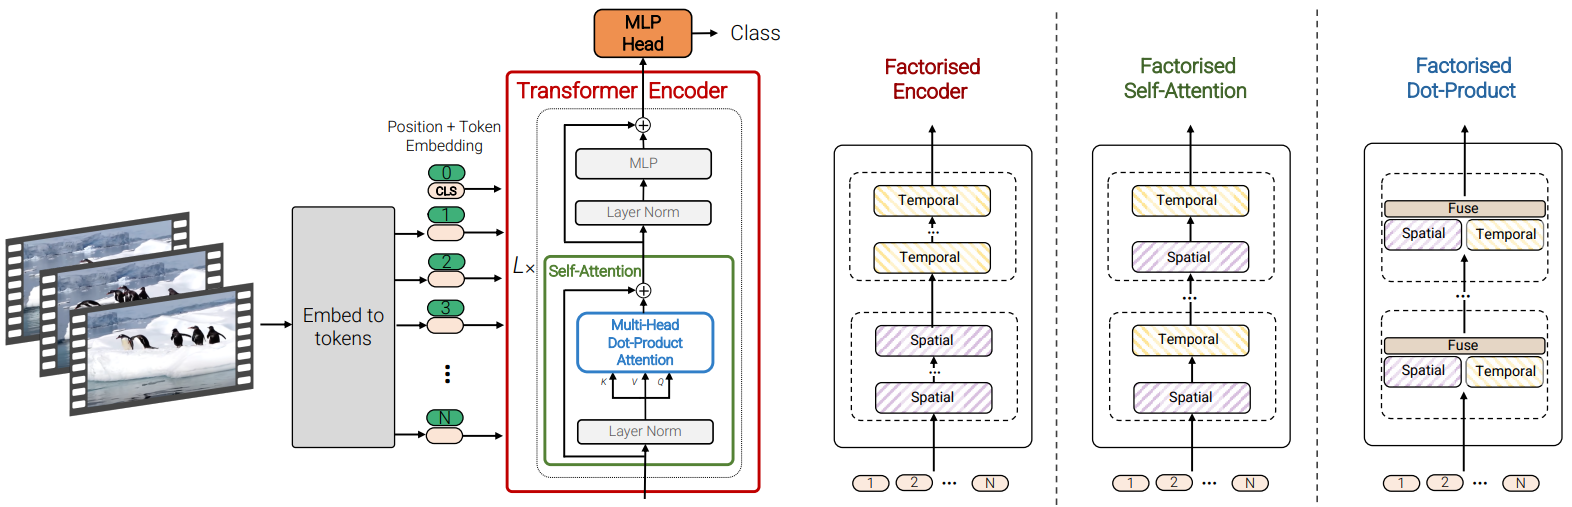
\includegraphics[width=0.75\textwidth]{figure/Vivit.png}}
	\caption{Arsitektur ViViT \cite{Arnab2021}.}
	\label{fig:vivit-architecture}
\end{figure}

Bobot pra-latih ViViT diinisialisasi dari \textit{checkpoint} ViT yang dilatih pada ImageNet, kemudian dilanjutkan dengan pra-latih \textit{supervised} pada dataset video berskala besar seperti Kinetics-400 \cite{Arnab2021}. Strategi ini berbeda dari VideoMAE yang mengandalkan pra-latih \textit{self-supervised} tanpa label, menjadikan ViViT representasi dari paradigma \textit{supervised video pre-training} berbasis Transformer. Dengan demikian, ketiga model dalam penelitian ini mencakup tiga paradigma yang berbeda secara metodologi: 3D CNN \textit{supervised} (I3D), Transformer \textit{supervised} (ViViT), dan Transformer \textit{self-supervised} (VideoMAE) \cite{Arnab2021,Tong2022VideoMAE}.\par

\subsection{Model VideoMAE} \label{II.teori2.4}
Video Masked Autoencoder (VideoMAE) adalah kerangka \textit{self-supervised} untuk video yang belajar merekonstruksi piksel patch yang dimask dari cuplikan video tanpa label. Inti idenya adalah \textit{tube masking} dengan rasio sangat tinggi, misalnya 90 persen, sehingga encoder hanya melihat sebagian kecil token dan dipaksa mempelajari struktur spasio-temporal yang benar-benar informatif \cite{Tong2022VideoMAE}. Arsitektur menggunakan \textit{encoder--decoder} asimetris berbasis ViT 3D, di mana encoder berkapasitas tinggi beroperasi pada token yang tampak, sedangkan decoder ringan merekonstruksi piksel pada lokasi yang disembunyikan \cite{Tong2022VideoMAE}. Versi lanjutan, VideoMAE~V2, memperkenalkan \textit{dual masking} untuk mengefisienkan komputasi dengan juga memasker sebagian input decoder menggunakan \textit{running-cell} sehingga beban memori dan FLOPs turun tanpa mengorbankan akurasi \cite{Wang2023VideoMAEv2}. Pendekatan ini terbukti data-efisien dan dapat diskalakan ke model berukuran miliar parameter pada beragam tugas hilir video \cite{Wang2023VideoMAEv2}.

\subsubsection{Konsep Dasar VideoMAE} \label{II.teori2.4.1}
VideoMAE mengadaptasi prinsip MAE pada citra ke domain video dengan menambahkan dimensi waktu sebagai token spasio-temporal. Gagasan ini berangkat dari keberhasilan Masked Autoencoders pada citra yang menunjukkan bahwa rekonstruksi patch termask mampu menghasilkan representasi visual yang kuat dan efisien \cite{He2022MAE}. Karena video memiliki redundansi temporal yang tinggi dan korelasi antarkader, \textit{tube masking} dengan peta masker yang sama di seluruh frame digunakan untuk mencegah \textit{information leakage} dan mendorong pembelajaran representasi yang lebih general \cite{Tong2022VideoMAE}. Dalam praktiknya, sekitar 90 persen patch kubus disembunyikan, lalu model meminimalkan \textit{mean squared error} antara piksel termask dan hasil rekonstruksi, sehingga sinyal latih tidak bergantung pada label \cite{Tong2022VideoMAE}. Berbeda dengan ViViT yang dilatih secara \textit{supervised} pada label aksi, VideoMAE mempelajari representasi dengan tugas generatif yang lebih murah label dan lebih mudah diskalakan \cite{Arnab2021,Tong2022VideoMAE}. Desain ini membuat VideoMAE efisien pada pra-latih besar karena encoder memproses hanya 10 persen token, sementara decoder yang ringan bertugas untuk rekonstruksi \cite{Tong2022VideoMAE}.

\subsubsection{Arsitektur VideoMAE} \label{II.teori2.4.2}
Arsitektur VideoMAE terdiri dari tiga komponen utama, yaitu \textit{cube embedding} sebagai pembentuk token, encoder ViT 3D dengan atensi ruang--waktu, serta decoder ringan untuk rekonstruksi piksel \cite{Tong2022VideoMAE}. Video dipotong menjadi token spasio-temporal berukuran $2 \times 16 \times 16$ dan diberi \textit{positional embedding} agar urutan ruang dan waktu tetap terjaga. Selama \textit{fine-tuning}, decoder dihapus dan kepala klasifikasi ringan ditambahkan pada representasi encoder mengikuti praktik ViT \cite{Dosovitskiy2021,Tong2022VideoMAE}. Skema umum arsitektur ini diilustrasikan pada Gambar~\ref{fig:videomae-architecture}.

\begin{figure}[h]
	\centering
	\fbox{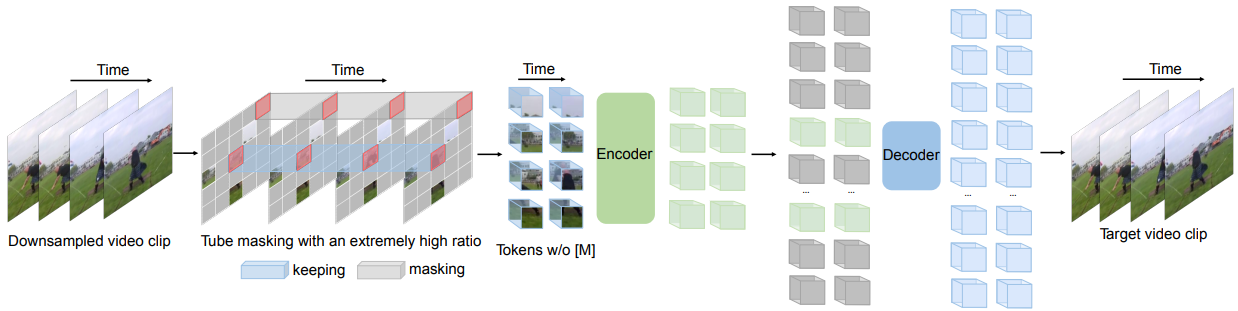
\includegraphics[width=0.75\textwidth]{figure/AlurVideoMAE.png}}
	\caption{Arsitektur VideoMAE \cite{Tong2022VideoMAE}.}
	\label{fig:videomae-architecture}
\end{figure}

Gambar~\ref{fig:videomae-architecture} memperlihatkan aliran token dari kubus video menuju encoder yang hanya memproses token tidak termask, kemudian decoder yang menggabungkan fitur encoder dengan token \texttt{[MASK]} untuk merekonstruksi piksel yang hilang. Penjelasan rinci masing-masing komponen diuraikan berikut.
\begin{enumerate}
\item Token spasio-temporal\\
Setiap klip dibagi menjadi kubus berukuran tetap yang dipetakan ke vektor token melalui \textit{cube embedding}. Proses ini menyatukan informasi ruang dan waktu menjadi barisan token yang dapat diproses oleh Transformer \cite{Tong2022VideoMAE}. Penambahan \textit{positional embedding} menjaga urutan temporal dan lokasi spasial selama atensi bersama \cite{Tong2022VideoMAE}. Representasi ini menjadi landasan untuk masking ekstrem dan rekonstruksi piksel \cite{Tong2022VideoMAE}.

\item Encoder ViT 3D\\
Encoder adalah ViT dengan \textit{joint space--time attention} yang hanya menerima token tidak termask. Karena panjang urutan encoder setara 10 persen dari token awal, biaya komputasi turun drastis tanpa kehilangan konteks global \cite{Tong2022VideoMAE}. Atensi multi-kepala memungkinkan pemodelan relasi antarframe dan antarpiksel yang jauh secara efisien \cite{Tong2022VideoMAE}. Hasil encoder berupa representasi laten yang kaya untuk berbagai tugas hilir \cite{Tong2022VideoMAE}.

\item Decoder ringan dan rekonstruksi\\
Decoder menerima gabungan fitur encoder dan token [MASK] lalu merekonstruksi piksel pada lokasi yang hilang. Fungsi kerugian yang digunakan adalah \textit{mean squared error} pada piksel termask yang dinormalisasi, sehingga gradien fokus pada area yang tidak terlihat encoder \cite{Tong2022VideoMAE}. Pada VideoMAE~V2, sebagian token untuk decoder juga dipilih selektif dengan \textit{running-cell masking} sehingga rekonstruksi tetap representatif tetapi lebih hemat memori \cite{Wang2023VideoMAEv2}. Strategi ini menyeimbangkan ketepatan dan efisiensi saat pra-latih skala besar \cite{Wang2023VideoMAEv2}.

\item Dual masking pada V2\\
Skema \textit{dual masking} menghasilkan dua peta masker berbeda untuk encoder dan decoder dengan rasio yang dapat diatur. Encoder tetap memakai \textit{tube masking} rasio sangat tinggi untuk mencegah kebocoran informasi temporal, sedangkan decoder memakai \textit{running-cell masking} untuk meliputi potongan video yang beragam \cite{Wang2023VideoMAEv2}. Hasilnya, panjang urutan decoder turun dan efisiensi meningkat tanpa menurunkan akurasi \cite{Wang2023VideoMAEv2}. Uji ablation menunjukkan rasio masker decoder 50 persen memberi titik tengah yang baik antara akurasi dan biaya \cite{Wang2023VideoMAEv2}.
\end{enumerate}

\subsubsection{Tahapan Pelatihan} \label{II.teori2.4.3}
Pelatihan VideoMAE umumnya dilakukan dua tahap, yaitu pra-latih \textit{self-supervised} dengan tugas rekonstruksi piksel, lalu \textit{fine-tuning} berlabel untuk tugas target. Pada pra-latih, model memaksimalkan kualitas rekonstruksi area termask menggunakan MSE Loss sehingga belajar merepresentasikan struktur gerak dan tampilan tanpa anotasi \cite{Tong2022VideoMAE}. Pada \textit{fine-tuning}, decoder dihapus dan kepala klasifikasi ditambahkan ke encoder untuk memetakan representasi menjadi label aksi atau isyarat \cite{Tong2022VideoMAE}. VideoMAE~V2 menambahkan \textit{post-pretraining} pada campuran data berlabel untuk stabilitas saat skala besar, tetapi efektivitasnya bergantung domain dan tidak selalu unggul pada semua dataset \cite{Wang2023VideoMAEv2}.

\begin{enumerate}
\item Pra-latih tanpa label\\
Model dilatih merekonstruksi piksel dari klip yang sebagian besar dimask, memaksa encoder mempelajari pola spasio-temporal. Strategi ini terbukti melampaui metode kontrasif pada aksi populer dan dapat dilatih efektif bahkan dengan korpus yang relatif kecil \cite{Tong2022VideoMAE}. Efek domain juga penting, sehingga kualitas dan kesesuaian data pra-latih terhadap target berdampak nyata pada transferabilitas \cite{Tong2022VideoMAE}. Hasil komparatif menunjukkan \textit{self-supervised} VideoMAE unggul pada Kinetics-400 dan SSV2 setelah \textit{fine-tuning} \cite{Tong2022VideoMAE}.

\item \textit{Fine-tuning} untuk klasifikasi\\
Setelah pra-latih, encoder diadaptasi dengan menambahkan kepala klasifikasi dan dioptimasi pada label tugas. Pada arsitektur encoder-saja seperti VideoMAE, ini setara pendekatan ViT dengan token \texttt{[CLS]} atau \textit{average pooling} representasi \cite{Dosovitskiy2021}. Prosedur ini menghasilkan peningkatan besar terhadap pelatihan dari nol, serta kompetitif dengan model \textit{supervised} skala besar \cite{Wang2023VideoMAEv2}. Praktik umum menggunakan Kinetics-400 atau Something-Something~V2 sebagai korpus rujukan untuk evaluasi \cite{Wang2023VideoMAEv2}.

\item \textit{Loss function}\\
Kerugian utama adalah \textit{mean squared error} antara piksel termask yang dinormalisasi dan hasil rekonstruksi. Penilaian hanya diterapkan pada token yang tidak terlihat encoder untuk menghindari kebocoran informasi dan memfokuskan pembelajaran pada area hilang \cite{Tong2022VideoMAE,Wang2023VideoMAEv2}. Skema ini sederhana, stabil, dan cocok untuk pra-latih skala besar. Penelitian lanjutan mengeksplorasi target lain, namun MSE pada piksel tetap menjadi dasar VideoMAE \cite{Tong2022VideoMAE}.

\item Dataset acuan\\
Evaluasi umum dilakukan pada Kinetics-400/600 untuk aksi generik dan Something-Something V1/V2 untuk interaksi berbasis objek, yang menuntut sensitivitas terhadap gerak halus \cite{Wang2023VideoMAEv2}. VideoMAE V2 menunjukkan hasil unggul pada benchmark tersebut tanpa data berlabel tambahan rumah-tangga, dan kompetitif dengan model besar yang dilatih \textit{supervised} \cite{Wang2023VideoMAEv2}. Selain itu, transfer ke deteksi aksi AVA menunjukkan representasi yang terlatih dapat digeneralisasi ke tugas yang lebih kompleks \cite{Tong2022VideoMAE}. Temuan ini menegaskan kelayakan pra-latih generatif untuk ragam aplikasi video.
\end{enumerate}

\subsection{Confusion Matrix} \label{II.Teori5}
Confusion matrix adalah metode dasar untuk mengevaluasi kinerja model klasifikasi, terutama dalam penelitian berbasis pembelajaran mesin seperti pengenalan isyarat tangan atau penerjemahan bahasa isyarat ke teks. Konsep ini digunakan untuk membandingkan hasil prediksi model terhadap label sebenarnya, sehingga dapat diketahui seberapa sering model membuat keputusan yang benar atau salah \cite{Raschka2020}. Matriks ini menggambarkan hubungan antara prediksi dan data aktual, membantu peneliti memahami jenis kesalahan yang dilakukan oleh model, misalnya apakah sistem sering salah mengenali tanda ``A'' sebagai ``E'' atau sebaliknya.\par

Pada penelitian ini, model dilatih untuk mengenali lebih dari dua kategori isyarat sekaligus, sehingga confusion matrix yang digunakan berbentuk \textit{multiclass} dengan ukuran $K \times K$, dengan $K$ menyatakan jumlah kelas dalam dataset \cite{Raschka2020}. Setiap sel $n_{ij}$ pada matriks menyatakan banyaknya sampel yang diprediksi oleh model sebagai kelas $i$ dan aktualnya berasal dari kelas $j$. Nilai pada diagonal utama ($n_{ii}$) menggambarkan jumlah prediksi yang benar untuk masing-masing kelas, sedangkan nilai di luar diagonal ($n_{ij}$ dengan $i \neq j$) menunjukkan kesalahan klasifikasi antar-kelas. Format ini lebih informatif dibandingkan matriks biner karena memperlihatkan pasangan kelas mana yang paling sering saling tertukar, sehingga dalam konteks bahasa isyarat dapat membantu mengidentifikasi isyarat dengan bentuk tangan atau arah gerak yang mirip.\par

\begin{table}[H]
	\caption{Confusion Matrix untuk Klasifikasi Multiclass dengan $K$ kelas}
	\label{tab:confusion-matrix-multiclass}
\centering
\begingroup
\setlength{\tabcolsep}{8pt}
\renewcommand{\arraystretch}{1.4}
	\begin{tabular}{|>{\centering\arraybackslash}m{1.8cm}|>{\centering\arraybackslash}m{1.2cm}|>{\centering\arraybackslash}m{1.2cm}|>{\centering\arraybackslash}m{1.2cm}|>{\centering\arraybackslash}m{1.2cm}|>{\centering\arraybackslash}m{1.2cm}|}
		\hline
		\rowcolor{gray!15}
		\multirow{2}{*}{\textbf{Prediksi}} & \multicolumn{5}{c|}{\textbf{Aktual}} \\ \cline{2-6}
		\rowcolor{gray!15}
		 & $\boldsymbol{C_1}$ & $\boldsymbol{C_2}$ & $\boldsymbol{C_3}$ & $\boldsymbol{\cdots}$ & $\boldsymbol{C_K}$ \\ \hline
		$C_1$ & $n_{11}$ & $n_{12}$ & $n_{13}$ & $\cdots$ & $n_{1K}$ \\ \hline
		$C_2$ & $n_{21}$ & $n_{22}$ & $n_{23}$ & $\cdots$ & $n_{2K}$ \\ \hline
		$C_3$ & $n_{31}$ & $n_{32}$ & $n_{33}$ & $\cdots$ & $n_{3K}$ \\ \hline
		$\vdots$ & $\vdots$ & $\vdots$ & $\vdots$ & $\ddots$ & $\vdots$ \\ \hline
		$C_K$ & $n_{K1}$ & $n_{K2}$ & $n_{K3}$ & $\cdots$ & $n_{KK}$ \\ \hline
	\end{tabular}
\endgroup
\end{table}

Untuk menurunkan metrik evaluasi dari confusion matrix multiclass, setiap kelas dianalisis dengan pendekatan \textit{one-vs-rest}, yaitu satu kelas dianggap sebagai kelas positif sedangkan gabungan seluruh kelas lainnya dianggap sebagai kelas negatif \cite{Raschka2020}. Dengan skema ini, empat komponen klasik \textit{True Positive} (TP), \textit{False Positive} (FP), \textit{False Negative} (FN), dan \textit{True Negative} (TN) dapat didefinisikan per kelas $i$ sebagai berikut:

\begin{itemize}
	\item $TP_i = n_{ii}$, jumlah sampel kelas $i$ yang diprediksi benar sebagai kelas $i$,
	\item $FP_i = \sum_{j \neq i} n_{ij}$, jumlah sampel bukan kelas $i$ yang keliru diprediksi sebagai kelas $i$,
	\item $FN_i = \sum_{j \neq i} n_{ji}$, jumlah sampel kelas $i$ yang keliru diprediksi sebagai kelas lain,
	\item $TN_i = N - TP_i - FP_i - FN_i$, dengan $N$ total seluruh sampel, yaitu sampel yang aktualnya bukan kelas $i$ dan juga tidak diprediksi sebagai kelas $i$.
\end{itemize}

Keempat komponen tersebut menjadi dasar untuk menghitung metrik akurasi, \textit{precision}, \textit{recall}, \textit{F1-score}, dan \textit{specificity} secara per-kelas. Agar diperoleh satu nilai ringkas yang menggambarkan performa model pada seluruh kelas, metrik per-kelas biasanya diagregasi menggunakan skema \textit{macro-average} yang memberi bobot sama untuk setiap kelas, atau \textit{weighted-average} yang membobot tiap kelas sesuai jumlah sampelnya \cite{Raschka2020}. \textit{Macro-average} cocok untuk dataset yang relatif seimbang, sedangkan \textit{weighted-average} lebih representatif ketika distribusi sampel antar-kelas tidak merata.\par

\begin{enumerate}
	\item Akurasi \\
	Akurasi pada klasifikasi multiclass mengukur proporsi seluruh sampel yang diprediksi benar dibandingkan dengan total data uji \cite{Raschka2020}. Nilai ini diperoleh dengan menjumlahkan seluruh elemen diagonal utama confusion matrix lalu membaginya dengan total sampel. Akurasi memberi gambaran umum kinerja model secara keseluruhan, tetapi tidak membedakan jenis kesalahan antar-kelas sehingga kurang informatif ketika distribusi kelas tidak seimbang.\\
	\vspace{0.5cm}
	\begin{equationcaptioned}[eq:2.accuracy]{
		Accuracy = \frac{\sum_{i=1}^{K} n_{ii}}{N} = \frac{\sum_{i=1}^{K} TP_i}{N}
	}{
		Rumus perhitungan akurasi pada klasifikasi multiclass
	}\end{equationcaptioned}
	\vspace{0.5cm}

	\noindent Keterangan:

	\begin{tabular}{@{}ll}
	$K$ & : jumlah kelas dalam dataset, \\
	$n_{ii}$ & : jumlah prediksi benar untuk kelas ke-$i$ (elemen diagonal matriks), \\
	$TP_i$ & : \textit{True Positive} kelas ke-$i$, \\
	$N$ & : total seluruh sampel pada data uji. \\
	\end{tabular}

	\vspace{0.5cm}
	Dalam konteks pengenalan bahasa isyarat, akurasi menunjukkan seberapa sering sistem mampu mengenali gerakan tangan dengan benar di seluruh kelas isyarat. Namun, jika jumlah sampel antar-isyarat tidak seimbang, akurasi dapat menyesatkan karena model bisa terlihat baik hanya dengan sering memprediksi kelas mayoritas. Oleh karena itu, akurasi sebaiknya digunakan bersama metrik per-kelas seperti \textit{precision} dan \textit{recall} \cite{Raschka2020}.\par


	\item Precision \\
	\textit{Precision} pada klasifikasi multiclass dihitung per kelas dengan memperlakukan satu kelas sebagai positif dan kelas lainnya sebagai negatif \cite{Raschka2020}. Nilai ini menunjukkan seberapa sering prediksi model untuk kelas tertentu benar-benar sesuai dengan label aslinya. Dalam konteks bahasa isyarat, \textit{precision} tinggi berarti sistem jarang salah melabeli sebuah gerakan sebagai isyarat yang bukan seharusnya, sehingga hasil terjemahan lebih dapat dipercaya.\par

	\vspace{0.5cm}
	\begin{equationcaptioned}[eq:2.precision]{
		\mathrm{Precision}_i &= \frac{\mathrm{TP}_i}{\mathrm{TP}_i + \mathrm{FP}_i} \\
		\mathrm{Precision}_{\mathrm{macro}} &= \frac{1}{K}\sum_{i=1}^{K} \mathrm{Precision}_i
	}{
		Rumus perhitungan \textit{precision} per kelas dan \textit{macro-average precision}
	}\end{equationcaptioned}
	\vspace{0.5cm}

	\noindent Keterangan:

	\begin{tabular}{@{}ll}
	$\mathrm{TP}_i$ & : jumlah prediksi benar untuk kelas ke-$i$, \\
	$\mathrm{FP}_i$ & : jumlah sampel bukan kelas $i$ yang salah diprediksi sebagai kelas $i$, \\
	$K$ & : jumlah kelas dalam dataset. \\
	\end{tabular}

	\vspace{0.5cm}
	\textit{Precision} per kelas berguna untuk mengetahui kelas mana yang paling sering mendapat prediksi salah dari kelas lain, sedangkan \textit{macro-precision} memberikan ringkasan tunggal yang adil antar kelas tanpa memperhitungkan dominasi kelas mayoritas \cite{Raschka2020}.\par

	\item Recall \\
	\textit{Recall}, juga dikenal sebagai sensitivitas, mengukur kemampuan model dalam mendeteksi seluruh sampel dari sebuah kelas secara benar \cite{Raschka2020}. Pada klasifikasi multiclass, \textit{recall} dihitung per kelas dengan membandingkan banyaknya prediksi benar kelas $i$ terhadap seluruh sampel yang sebenarnya berasal dari kelas $i$. Pada sistem penerjemahan bahasa isyarat, \textit{recall} tinggi berarti model mampu menangkap hampir semua kemunculan suatu isyarat meskipun variasinya berbeda.\par
	\vspace{0.5cm}
	\begin{equationcaptioned}[eq:2.recall]{
		\mathrm{Recall}_i &= \frac{\mathrm{TP}_i}{\mathrm{TP}_i + \mathrm{FN}_i} \\
		\mathrm{Recall}_{\mathrm{macro}} &= \frac{1}{K}\sum_{i=1}^{K} \mathrm{Recall}_i
	}{
		Rumus perhitungan \textit{recall} per kelas dan \textit{macro-average recall}
	}\end{equationcaptioned}
	\vspace{0.5cm}

	\noindent Keterangan:

	\begin{tabular}{@{}ll}
	$\mathrm{TP}_i$ & : jumlah sampel kelas ke-$i$ yang benar terdeteksi, \\
	$\mathrm{FN}_i$ & : jumlah sampel kelas ke-$i$ yang salah diprediksi sebagai kelas lain, \\
	$K$ & : jumlah kelas dalam dataset. \\
	\end{tabular}

	\vspace{0.5cm}
	\textit{Recall} yang rendah pada suatu kelas menandakan bahwa model sering melewatkan isyarat tersebut, sehingga dapat menjadi petunjuk kelas mana yang perlu ditambah data latih atau mendapat augmentasi khusus \cite{Raschka2020}.\par

	\item F1-Score \\
	F1-score menggabungkan \textit{precision} dan \textit{recall} menjadi satu ukuran tunggal berupa rata-rata harmonik keduanya, sehingga mencerminkan keseimbangan antara ketepatan dan kelengkapan deteksi \cite{Raschka2020}. Pada klasifikasi multiclass, F1-score dihitung per kelas terlebih dahulu lalu diagregasi dengan skema \textit{macro} atau \textit{weighted} seperti metrik lainnya. F1-score sangat relevan pada kasus data tidak seimbang, di mana akurasi saja tidak cukup menggambarkan performa model per-kelas.\par
	\vspace{0.5cm}
	\begin{equationcaptioned}[eq:2.f1]{
		\mathrm{F1}_i &= 2 \times \frac{\mathrm{Precision}_i \times \mathrm{Recall}_i}{\mathrm{Precision}_i + \mathrm{Recall}_i} \\
		\mathrm{F1}_{\mathrm{macro}} &= \frac{1}{K}\sum_{i=1}^{K} \mathrm{F1}_i
	}{
		Rumus perhitungan F1-score per kelas dan \textit{macro-average F1-score}
	}\end{equationcaptioned}
	\vspace{0.5cm}

	\noindent Keterangan:

	\begin{tabular}{@{}ll}
	$\mathrm{Precision}_i$ & : tingkat ketepatan prediksi untuk kelas ke-$i$, \\
	$\mathrm{Recall}_i$ & : tingkat keberhasilan model mendeteksi kelas ke-$i$, \\
	$K$ & : jumlah kelas dalam dataset. \\
	\end{tabular}

	\vspace{0.5cm}
	Sebagai rata-rata harmonik, F1-score memberikan penalti besar terhadap perbedaan ekstrem antara \textit{precision} dan \textit{recall}. Dalam pengenalan bahasa isyarat, nilai F1 yang tinggi pada semua kelas menunjukkan bahwa model mampu mengenali beragam isyarat secara konsisten tanpa bias terhadap kelas tertentu. Oleh karena itu, \textit{macro F1-score} sering dijadikan indikator utama kinerja sistem klasifikasi multiclass bahasa isyarat \cite{Raschka2020}.\par

	\item Specificity \\
	\textit{Specificity} atau \textit{true negative rate} pada klasifikasi multiclass dihitung per kelas dengan mengukur proporsi sampel bukan kelas $i$ yang berhasil dikenali sebagai bukan kelas $i$ oleh model \cite{Raschka2020}. Nilai \textit{specificity} yang tinggi untuk kelas tertentu berarti model jarang salah memasukkan gerakan dari kelas lain ke dalam kelas tersebut.\par

	\vspace{0.5cm}
	\begin{equationcaptioned}[eq:2.specificity]{
		\mathrm{Specificity}_i &= \frac{\mathrm{TN}_i}{\mathrm{TN}_i + \mathrm{FP}_i} \\
		\mathrm{Specificity}_{\mathrm{macro}} &= \frac{1}{K}\sum_{i=1}^{K} \mathrm{Specificity}_i
	}{
		Rumus perhitungan \textit{specificity} per kelas dan \textit{macro-average specificity}
	}\end{equationcaptioned}
	\vspace{0.5cm}

	\noindent Keterangan:

	\begin{tabular}{@{}ll}
	$\mathrm{TN}_i$ & : jumlah sampel bukan kelas $i$ yang benar diklasifikasikan sebagai bukan kelas $i$, \\
	$\mathrm{FP}_i$ & : jumlah sampel bukan kelas $i$ yang salah diklasifikasikan sebagai kelas $i$, \\
	$K$ & : jumlah kelas dalam dataset. \\
	\end{tabular}

	\vspace{0.5cm}
	Dalam konteks penerjemahan bahasa isyarat, \textit{specificity} yang tinggi per kelas membantu mengurangi kesalahan interpretasi dari isyarat lain yang memiliki bentuk tangan serupa. Metrik ini sering digunakan bersamaan dengan \textit{recall} untuk memberikan gambaran menyeluruh mengenai kemampuan sistem mengenali kelas yang benar sekaligus menolak kelas yang tidak relevan \cite{Raschka2020}.\par

\end{enumerate}
 
\subsection{Stratified Cross-Validation} \label{II.SCV}
\noindent\begin{figure}[H]
	\centering
	% Ilustrasi Stratified 5-Fold Cross-Validation

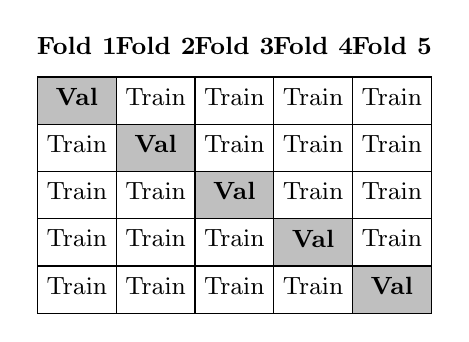
\begin{tikzpicture}[scale=1]
    \def\cellwidth{1.0}
    \def\cellheight{0.6}
    
    % Baris pertama (header dengan Fold 1-5)
    \foreach \i in {1,2,3,4,5} {
        \node[font=\small\bfseries] at (\i*\cellwidth - 0.5, 3.2) {Fold \i};
    }
    
    % 5 baris data
    \foreach \row in {0,1,2,3,4} {
        \foreach \col in {1,2,3,4,5} {
            \pgfmathparse{\col == \row + 1 ? 1 : 0}
            \ifnum\pgfmathresult=1
                % Validation fold (gray)
                \draw[fill=gray!50] (\col*\cellwidth - 1, 2.8 - \row*\cellheight) rectangle (\col*\cellwidth - 1 + \cellwidth, 2.8 - \row*\cellheight - \cellheight);
                \node[font=\small\bfseries] at (\col*\cellwidth - 0.5, 2.55 - \row*\cellheight) {Val};
            \else
                % Training fold (white)
                \draw[fill=white] (\col*\cellwidth - 1, 2.8 - \row*\cellheight) rectangle (\col*\cellwidth - 1 + \cellwidth, 2.8 - \row*\cellheight - \cellheight);
                \node[font=\small] at (\col*\cellwidth - 0.5, 2.55 - \row*\cellheight) {Train};
            \fi
            \draw[black, line width=0.5pt] (\col*\cellwidth - 1, 2.8 - \row*\cellheight) rectangle (\col*\cellwidth - 1 + \cellwidth, 2.8 - \row*\cellheight - \cellheight);
        }
    }
    
\end{tikzpicture}

	\caption{Ilustrasi Stratified Cross-Validation}
	\label{fig:II.stratified_kfold}
\end{figure}
\textit{Stratified Cross-Validation} (SCV) merupakan skema validasi yang membagi data ke dalam beberapa \textit{fold} sambil mempertahankan proporsi kelas yang relatif sama pada setiap bagian data. Pendekatan ini penting ketika distribusi kelas tidak seimbang, karena pembagian acak biasa dapat menghasilkan subset yang terlalu didominasi kelas tertentu dan membuat evaluasi menjadi bias \cite{Raschka2020}. Dengan menjaga komposisi label tetap proporsional, SCV memberikan estimasi performa yang lebih stabil dan lebih representatif terhadap kemampuan generalisasi model pada data baru \cite{Raschka2020}.

Dalam praktik pembelajaran mesin, SCV umum digunakan bersama metrik evaluasi seperti akurasi, presisi, recall, dan F1-score agar penilaian model tidak hanya bergantung pada satu pembagian data. Untuk dataset bahasa isyarat yang relatif kecil, strategi ini membantu memanfaatkan data secara lebih efisien sekaligus menjaga konsistensi evaluasi antar percobaan \cite{Raschka2020}. Dengan demikian, SCV menjadi prosedur validasi yang relevan untuk tugas klasifikasi gerakan visual yang memiliki variasi kelas dan jumlah sampel yang tidak selalu seimbang.
